% ============================================================================
% MILO — Consumer Panel & Market Intelligence Platform Business Plan (v3.1)
% Panelist App & B2B Data Products for the Belgian FMCG Industry
% ============================================================================
\documentclass[11pt,a4paper]{article}

% --- Core Packages ---
\usepackage[utf8]{inputenc}
\usepackage[T1]{fontenc}
\usepackage[english]{babel}
\usepackage{geometry}
\usepackage{graphicx}
\usepackage{xcolor}
\usepackage{tikz}
\usepackage{tabularx}
\usepackage{booktabs}
\usepackage{enumitem}
\usepackage{fancyhdr}
\usepackage{titlesec}
\usepackage{hyperref}
\usepackage{fontspec}
\usepackage{setspace}
\usepackage{parskip}
\usepackage{multicol}
\usepackage{float}
\usepackage{colortbl}
\usepackage{array}
\usepackage{calc}
\usepackage{etoolbox}
\usepackage{tcolorbox}
\usepackage{pgfplots}
\usepackage{makecell}
\usepackage{lastpage}
\usepackage{ragged2e}
\usepackage{microtype}
\usepackage{needspace}

\tcbuselibrary{skins,breakable}
\pgfplotsset{compat=1.18}
\usetikzlibrary{calc,positioning,shapes.geometric,arrows.meta,patterns,decorations.markings,shadows}

% --- Page Geometry ---
\geometry{
  a4paper,
  top=2.5cm,
  bottom=2.5cm,
  left=2.5cm,
  right=2.5cm,
  headheight=1.5cm,
  headsep=0.8cm,
  footskip=1.2cm
}

% ============================================================================
% PREMIUM COLOR PALETTE
% ============================================================================
\definecolor{milodark}{HTML}{1B1A35}
\definecolor{miloprimary}{HTML}{2E5266}
\definecolor{miloaccent}{HTML}{6AB0A0}
\definecolor{milowarm}{HTML}{C08B5C}
\definecolor{milolightbg}{HTML}{F5F2ED}
\definecolor{milogray}{HTML}{5F6B7A}
\definecolor{milolightgray}{HTML}{E2DED8}
\definecolor{milogreen}{HTML}{5DAE72}
\definecolor{milored}{HTML}{D46B5D}
\definecolor{miloblue}{HTML}{5B8DB8}
\definecolor{milowarmlight}{HTML}{F0E6D6}
\definecolor{tabheader}{HTML}{2E5266}
\definecolor{tabrow}{HTML}{EEEAE4}
\definecolor{milodarker}{HTML}{12112A}
\definecolor{milogold}{HTML}{FFD600}
\definecolor{milopurple}{HTML}{7C5CBF}

% --- Fonts ---
\setmainfont{TeX Gyre Heros}

% --- Hyperlinks ---
\hypersetup{
  colorlinks=true,
  linkcolor=miloprimary,
  urlcolor=miloprimary,
  citecolor=miloprimary,
  pdfauthor={Milo},
  pdftitle={Milo - Consumer Panel and Market Intelligence Platform},
  pdfsubject={Panelist App and B2B Data Products for Belgian FMCG},
}

% --- Header & Footer ---
\pagestyle{fancy}
\fancyhf{}
\renewcommand{\headrulewidth}{0pt}
\renewcommand{\footrulewidth}{0pt}

% Explicitly define empty pagestyle so TikZ overlay headers never bleed onto cover/closing pages
\fancypagestyle{empty}{%
  \fancyhf{}%
  \renewcommand{\headrulewidth}{0pt}%
  \renewcommand{\footrulewidth}{0pt}%
}

\fancyhead[L]{%
  \begin{tikzpicture}[remember picture, overlay]
    \fill[milodark] ([yshift=0.2cm]current page.north west) rectangle ([yshift=-1.3cm, xshift=\paperwidth]current page.north west);
    \node[anchor=west, inner sep=0pt] at ([xshift=2.5cm, yshift=-0.55cm]current page.north west) {%
      
\includegraphics[height=0.8cm]{milo-logo.png}%
    };
    \node[anchor=west, text=white, font=\fontsize{9}{11}\selectfont\bfseries, inner sep=0pt] at ([xshift=3.6cm, yshift=-0.45cm]current page.north west) {MILO};
    \node[anchor=west, text=miloaccent, font=\fontsize{7}{9}\selectfont, inner sep=0pt] at ([xshift=3.6cm, yshift=-0.75cm]current page.north west) {Consumer Panel \& Market Intelligence Platform};
    \node[anchor=east, text=white!70, font=\fontsize{7}{9}\selectfont, inner sep=0pt] at ([xshift=-2.5cm, yshift=-0.55cm]current page.north east) {CONFIDENTIAL};
  \end{tikzpicture}%
}
\fancyfoot[C]{%
  \begin{tikzpicture}[remember picture, overlay]
    \fill[milodark] ([yshift=1cm]current page.south west) rectangle (current page.south east);
    \node[text=white!60, font=\fontsize{7}{9}\selectfont] at ([yshift=0.5cm]current page.south) {%
      \thepage\ / \pageref{LastPage} \quad\textbar\quad Milo --- Consumer Panel \& Market Intelligence Platform \quad\textbar\quad March 2026%
    };
  \end{tikzpicture}%
}

% --- Section Styling ---
\titleformat{\section}
  {\color{milodark}\fontsize{20}{24}\selectfont\bfseries}
  {\thesection.}{0.5em}{}
  [\vspace{-0.3em}{\color{miloaccent}\rule{\textwidth}{2pt}}]

\titleformat{\subsection}
  {\color{miloprimary}\fontsize{14}{17}\selectfont\bfseries}
  {\thesubsection}{0.5em}{}

\titleformat{\subsubsection}
  {\color{miloprimary}\fontsize{12}{14}\selectfont\bfseries}
  {\thesubsubsection}{0.5em}{}

\titlespacing*{\section}{0pt}{1.5em}{0.8em}
\titlespacing*{\subsection}{0pt}{1em}{0.5em}
\titlespacing*{\subsubsection}{0pt}{0.8em}{0.3em}

% --- Custom Environments ---
\newtcolorbox{milobox}[1][]{
  enhanced,
  colback=milolightbg,
  colframe=miloprimary,
  boxrule=0.5pt,
  arc=4pt,
  left=12pt,
  right=12pt,
  top=10pt,
  bottom=10pt,
  fonttitle=\bfseries\color{white},
  coltitle=white,
  colbacktitle=miloprimary,
  attach boxed title to top left={yshift=-2mm, xshift=5mm},
  boxed title style={arc=3pt, boxrule=0pt},
  #1
}

\newtcolorbox{keymetric}[1][]{
  enhanced,
  colback=white,
  colframe=miloaccent,
  boxrule=1.5pt,
  arc=6pt,
  left=10pt,
  right=10pt,
  top=8pt,
  bottom=8pt,
  #1
}

\newtcolorbox{productbox}[1][]{
  enhanced,
  breakable,
  colback=white,
  colframe=milolightgray,
  boxrule=0.5pt,
  arc=4pt,
  left=12pt,
  right=12pt,
  top=10pt,
  bottom=10pt,
  shadow={0.5mm}{-0.5mm}{0mm}{black!8},
  borderline west={3pt}{0pt}{miloprimary},
  #1
}

\newtcolorbox{qabox}[1][]{
  enhanced,
  colback=milolightbg,
  colframe=milolightgray,
  boxrule=0.3pt,
  arc=3pt,
  left=10pt,
  right=10pt,
  top=8pt,
  bottom=8pt,
  borderline west={2pt}{0pt}{miloaccent},
  #1
}

\newtcolorbox{alertbox}[1][]{
  enhanced,
  colback=milowarmlight,
  colframe=milowarm,
  boxrule=0.5pt,
  arc=4pt,
  left=12pt,
  right=12pt,
  top=8pt,
  bottom=8pt,
  #1
}

\newtcolorbox{premiumbox}[1][]{
  enhanced,
  breakable,
  colback=milodark!5,
  colframe=milowarm,
  boxrule=1pt,
  arc=6pt,
  left=14pt,
  right=14pt,
  top=12pt,
  bottom=12pt,
  shadow={1mm}{-1mm}{0mm}{milowarm!15},
  #1
}

\newtcolorbox{categorybox}[1][]{
  enhanced,
  breakable,
  colback=white,
  colframe=miloaccent,
  boxrule=0.8pt,
  arc=5pt,
  left=12pt,
  right=12pt,
  top=10pt,
  bottom=10pt,
  shadow={0.5mm}{-0.5mm}{0mm}{miloaccent!10},
  borderline north={2.5pt}{0pt}{miloaccent},
  #1
}

\newtcolorbox{appbox}[1][]{
  enhanced,
  breakable,
  colback=milodark!3,
  colframe=milopurple!60,
  boxrule=0.8pt,
  arc=5pt,
  left=12pt,
  right=12pt,
  top=10pt,
  bottom=10pt,
  shadow={0.5mm}{-0.5mm}{0mm}{milopurple!8},
  borderline west={3pt}{0pt}{milopurple!60},
  #1
}

% --- Custom Commands ---
\newcommand{\sectionbreak}{\clearpage}

% --- Table Column Types ---
\newcolumntype{L}[1]{>{\raggedright\arraybackslash}p{#1}}
\newcolumntype{C}[1]{>{\centering\arraybackslash}p{#1}}
\newcolumntype{R}[1]{>{\raggedleft\arraybackslash}p{#1}}

% ============================================================================
% DOCUMENT START
% ============================================================================
\begin{document}
\thispagestyle{empty}

% ============================================================================
% COVER PAGE
% ============================================================================
\begin{tikzpicture}[remember picture, overlay]
  % Full page dark background
  \fill[milodark] (current page.south west) rectangle (current page.north east);

  % Subtle geometric pattern
  \foreach \i in {1,...,10} {
    \draw[white, opacity=0.02, line width=0.3pt]
      ([xshift=\i*2.1cm]current page.south west) -- ([xshift=\i*2.1cm-4cm]current page.north west);
  }
  \foreach \i in {1,...,15} {
    \draw[white, opacity=0.015, line width=0.3pt]
      ([yshift=\i*2cm]current page.south west) -- ([yshift=\i*2cm]current page.south east);
  }

  % Top accent line
  \fill[miloaccent] ([yshift=-0.6cm]current page.north west) rectangle ([yshift=-0.35cm]current page.north east);

  % Logo
  \node[anchor=center] at ([yshift=5.5cm]current page.center) {%
    
\includegraphics[width=4.5cm]{milo-logo.png}%
  };

  % Company name
  \node[anchor=center, text=white, font=\fontsize{52}{62}\selectfont\bfseries] at ([yshift=1.5cm]current page.center) {MILO};

  % Primary tagline
  \node[anchor=center, text=miloaccent, font=\fontsize{13}{17}\selectfont] at ([yshift=0.1cm]current page.center) {Consumer Panel \& Market Intelligence Platform for Belgian FMCG};

  % Subtitle
  \node[anchor=center, text=white!75, font=\fontsize{10.5}{14}\selectfont] at ([yshift=-1.2cm]current page.center) {%
    \begin{tabular}{c}
    A free panelist app that rewards consumers for submitting digital grocery receipts.\\[3pt]
    Two B2B data products that give brands the market intelligence they've never had.
    \end{tabular}
  };

  % Divider line
  \draw[milowarm, line width=0.8pt] ([xshift=5cm, yshift=-2.6cm]current page.center) -- ([xshift=-5cm, yshift=-2.6cm]current page.center);

  % Document type
  \node[anchor=center, text=white, font=\fontsize{15}{19}\selectfont\bfseries, text width=12cm, align=center] at ([yshift=-3.8cm]current page.center) {BUSINESS PLAN};

  % Date and Confidential
  \node[anchor=center, text=white!55, font=\fontsize{9.5}{12}\selectfont] at ([yshift=-5cm]current page.center) {March 2026 \quad\textbar\quad Confidential \quad\textbar\quad Version 3.1};

  % Bottom accent line
  \fill[miloaccent] ([yshift=0.35cm]current page.south west) rectangle ([yshift=0.6cm]current page.south east);
\end{tikzpicture}

\clearpage

% ============================================================================
% TABLE OF CONTENTS
% ============================================================================
\thispagestyle{fancy}

\vspace*{0.5cm}
{\color{milodark}\fontsize{28}{34}\selectfont\bfseries Table of Contents}\\[2pt]
{\color{miloaccent}\rule{6cm}{2pt}}

\vspace{1cm}
\renewcommand{\contentsname}{}
\setcounter{tocdepth}{2}
{
\hypersetup{linkcolor=milodark}
\tableofcontents
}

\clearpage

% ============================================================================
% 1. EXECUTIVE SUMMARY
% ============================================================================
\section{Executive Summary}

\begin{alertbox}
\textbf{\color{milodark}The Thesis:} Belgian consumers have no tool that turns grocery receipts into granular spending and health insights. Belgian FMCG brands have no affordable source of cross-retailer market data. \textbf{Milo solves both problems with one platform} --- a free panelist app that collects the data, and a B2B product that monetizes it.
\end{alertbox}

\vspace{0.5em}

\textbf{Milo} is a consumer panel and market intelligence platform for the Belgian grocery industry. Through a \textbf{completely free} mobile app, Belgian consumers submit their digital grocery receipts in exchange for real euro cashback rewards, while gaining item-level spending analytics, nutritional health scoring, and an AI financial coach. On the B2B side, this receipt data is matched to real product EANs via Daltix and aggregated into \textbf{two core data products}: \texttt{mart\_sku\_performance} (22 metrics at the EAN $\times$ store $\times$ month grain) and \texttt{mart\_brand\_switching} (a brand-to-brand transition matrix per category). Clients open these in Excel and pivot/filter --- giving them the cross-retailer competitive intelligence that didn't exist at an accessible price point.

The Milo app is not just a data collection tool --- it is a \textbf{full-featured consumer product} with a sophisticated gamification engine that drives long-term panelist retention. Because the app is entirely free, there is zero friction to adoption. This creates a self-reinforcing flywheel: better app $\rightarrow$ more panelists $\rightarrow$ richer data $\rightarrow$ more B2B revenue $\rightarrow$ more reward budget $\rightarrow$ better app.

\vspace{0.3em}

\begin{keymetric}
\begin{center}
\renewcommand{\arraystretch}{1.4}
\begin{tabular}{ccccc}
\textbf{\color{milodark}\fontsize{22}{26}\selectfont 100\%} &
\textbf{\color{milodark}\fontsize{22}{26}\selectfont 2} &
\textbf{\color{milodark}\fontsize{22}{26}\selectfont 22} &
\textbf{\color{milodark}\fontsize{22}{26}\selectfont 3,900+} &
\textbf{\color{milodark}\fontsize{22}{26}\selectfont 0} \\
{\scriptsize Free} & {\scriptsize Data} & {\scriptsize SKU Performance} & {\scriptsize Potential} & {\scriptsize Affordable Cross-} \\
{\scriptsize Consumer App} & {\scriptsize Products} & {\scriptsize Metrics} & {\scriptsize B2B Clients} & {\scriptsize Retailer Alternatives} \\
\end{tabular}
\end{center}
\end{keymetric}

\subsection{The Platform Flywheel}

\begin{center}
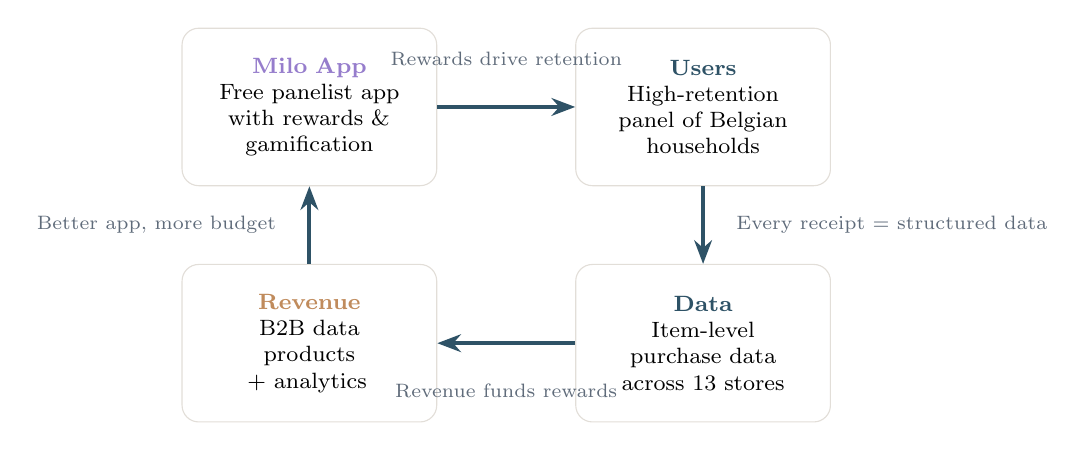
\begin{tikzpicture}[
  box/.style={fill=white, draw=milolightgray, rounded corners=6pt, minimum width=3.2cm, minimum height=2cm, align=center, font=\footnotesize, text width=3cm},
  arrow/.style={-{Stealth[length=3mm]}, miloprimary, line width=1.5pt},
  label/.style={font=\tiny\bfseries\color{miloprimary}, above=2pt}
]
  % Circular flywheel
  \node[box] (app) at (0,2.5) {\textbf{\color{milopurple!80}Milo App}\\Free panelist app\\with rewards \&\\gamification};
  \node[box] (users) at (5,2.5) {\textbf{\color{miloprimary}Users}\\High-retention\\panel of Belgian\\households};
  \node[box] (data) at (5,-0.5) {\textbf{\color{miloprimary}Data}\\Item-level\\purchase data\\across 13 stores};
  \node[box] (revenue) at (0,-0.5) {\textbf{\color{milowarm}Revenue}\\B2B data\\products\\+ analytics};

  \draw[arrow] (app) -- (users);
  \draw[arrow] (users) -- (data);
  \draw[arrow] (data) -- (revenue);
  \draw[arrow] (revenue) -- (app);

  \node[font=\scriptsize\color{milogray}, above=0pt] at (2.5,2.9) {Rewards drive retention};
  \node[font=\scriptsize\color{milogray}, right=0pt] at (5.3,1) {Every receipt = structured data};
  \node[font=\scriptsize\color{milogray}, below=0pt] at (2.5,-0.9) {Revenue funds rewards};
  \node[font=\scriptsize\color{milogray}, left=0pt] at (-0.3,1) {Better app, more budget};
\end{tikzpicture}
\end{center}

\subsection{Revenue Architecture}

\begin{center}
\renewcommand{\arraystretch}{1.3}
\begin{tabularx}{\textwidth}{L{3.5cm} R{3cm} L{7cm}}
\toprule
\rowcolor{tabheader}
\textbf{\color{white}Revenue Stream} & \textbf{\color{white}Price Range} & \textbf{\color{white}Description} \\
\midrule
SKU Performance Data & \texteuro{}149--799/mo & \texttt{mart\_sku\_performance}: 22 metrics at EAN $\times$ store $\times$ month grain \\
\rowcolor{tabrow}
Brand Switching Data & \texteuro{}199--599/mo & \texttt{mart\_brand\_switching}: loyalty \& switching matrix per category \\
Multi-Category Bundles & \texteuro{}380--4,500/mo & 3, 5, or 8 category bundles with volume discount \\
\rowcolor{tabrow}
Ad-Hoc Research & \texteuro{}2K--8K/project & Custom analysis on demand \\
Retailer Partnerships & Variable & Coupon sponsorship and promoted deal placements \\
\bottomrule
\end{tabularx}
\end{center}

\clearpage

% ============================================================================
% 2. THE MARKET OPPORTUNITY
% ============================================================================
\section{The Market Opportunity}

\subsection{Two Markets, One Platform}

Milo addresses two distinct market failures simultaneously:

\begin{premiumbox}
\begin{center}
\begin{minipage}[t]{0.42\textwidth}
\centering
{\color{milopurple!80}\fontsize{12}{14}\selectfont\bfseries Consumer Problem}

\vspace{0.4em}
{\footnotesize Expense trackers show ``\texteuro{}45 at Colruyt'' --- never \emph{what} you actually bought. No app combines item-level spending, health, AI coaching, and real cashback rewards.}

\vspace{0.3em}
{\color{milogray}\scriptsize\textbf{5.2M Belgian households}\textsuperscript{[1]} with no granular grocery spending tool}
\end{minipage}%
\hfill
\begin{minipage}[t]{0.1\textwidth}
\centering
\vspace{1.5em}
{\footnotesize\bfseries\color{milowarm}MILO\\SOLVES\\BOTH}
\end{minipage}%
\hfill
\begin{minipage}[t]{0.42\textwidth}
\centering
{\color{miloprimary}\fontsize{12}{14}\selectfont\bfseries B2B Data Problem}

\vspace{0.4em}
{\footnotesize 99\% of Belgium's 3,979 food companies\textsuperscript{[2]} have zero cross-retailer consumer data. YouGov costs \texteuro{}100K+/yr.\textsuperscript{[3]} Retailer data is siloed. No one offers SKU-level switching data.}

\vspace{0.3em}
{\color{milogray}\scriptsize\textbf{3,500+ companies}\textsuperscript{[2]} priced out of market intelligence entirely}
\end{minipage}
\end{center}
\end{premiumbox}

\subsection{The Consumer Market}

Belgian consumers are underserved by financial tracking tools. Bank-connected apps (like Cake, Bankin') only show merchant-level aggregates --- ``\texteuro{}45.23 at Colruyt'' tells you nothing about what you actually bought. \textbf{No app on the Belgian market} provides:

\begin{itemize}[leftmargin=1.5em, itemsep=3pt]
  \item \textbf{Item-level spending analytics} --- which products, at what price, in what category
  \item \textbf{Nutritional health scoring} of grocery purchases
  \item \textbf{AI-powered financial coaching} with full purchase history context
  \item \textbf{Real cashback rewards} (\texteuro{}0.50+ per receipt) that fund the habit
  \item \textbf{Personalized deal recommendations} based on actual purchase history
\end{itemize}

Post-inflation awareness (12--15\% food inflation in Belgium, 2022--2023\textsuperscript{[4]}) has created unprecedented demand for grocery budgeting tools. The Milo app meets this demand while building the data asset that powers the B2B business.

\subsection{The B2B Data Gap}

FMCG brands in Belgium are \textbf{flying blind}. They sell through Colruyt, Delhaize, Carrefour, Aldi, and Lidl --- but have no idea who buys their products, how often, or what happens at competing retailers.

\begin{center}
\renewcommand{\arraystretch}{1.3}
\begin{tabularx}{\textwidth}{L{2.6cm} C{1.6cm} C{1.6cm} C{1.8cm} C{1.5cm} C{1.6cm} C{1.6cm}}
\toprule
\rowcolor{tabheader}
\textbf{\color{white}Data Source} & \textbf{\color{white}Cross-Ret.?} & \textbf{\color{white}Purchase?} & \textbf{\color{white}Affordable?} & \textbf{\color{white}SKU?} & \textbf{\color{white}Switching?} & \textbf{\color{white}Basket?} \\
\midrule
YouGov\textsuperscript{[3]} & Yes & Yes & \textcolor{milored}{No (\texteuro{}100K+)} & Yes & Partial & Yes \\
\rowcolor{tabrow}
Colruyt Insights\textsuperscript{[7]} & \textcolor{milored}{No} & Yes & Unknown & Yes & \textcolor{milored}{No} & Yes \\
Delhaize Enlight+\textsuperscript{[8]} & \textcolor{milored}{No} & Yes & \textcolor{milored}{No} & Yes & \textcolor{milored}{No} & Yes \\
\rowcolor{tabrow}
Carrefour Links\textsuperscript{[9]} & \textcolor{milored}{No} & Yes & \textcolor{milored}{No} & Yes & \textcolor{milored}{No} & Yes \\
Shopmium\textsuperscript{[13]} & Yes & \textcolor{milored}{Biased} & N/A & \textcolor{milored}{No} & \textcolor{milored}{No} & \textcolor{milored}{No} \\
\rowcolor{tabrow}
\textbf{\color{miloprimary}Milo} & \textbf{\color{milogreen}Yes} & \textbf{\color{milogreen}Yes} & \textbf{\color{milogreen}Yes} & \textbf{\color{milogreen}Yes} & \textbf{\color{milogreen}Yes} & \textbf{\color{milogreen}Yes} \\
\bottomrule
\end{tabularx}
\end{center}

Retailers monetize their \emph{own} data but will \textbf{never share cross-retailer data}. Colruyt will never tell a brand what happens at Delhaize. This competitive dynamic is permanent and creates a structurally defensible market position for Milo.

\subsection{Total Addressable Market}

\begin{center}
\renewcommand{\arraystretch}{1.3}
\begin{tabularx}{\textwidth}{L{4cm} R{2.5cm} C{2.5cm} L{4.5cm}}
\toprule
\rowcolor{tabheader}
\textbf{\color{white}Segment} & \textbf{\color{white}Potential \texteuro{}/yr} & \textbf{\color{white}Companies} & \textbf{\color{white}Key Buyers} \\
\midrule
\multicolumn{4}{l}{\textbf{\color{miloprimary}\small B2B Data Products}} \\
\midrule
Belgian SMB food producers\textsuperscript{[2]} & \texteuro{}3.6M--8.4M & 3,400+ & Artisanal producers, local brands \\
\rowcolor{tabrow}
Mid-size Belgian brands & \texteuro{}3.6M--14.4M & 50--100 & Lotus, La William, Imperial \\
Market research agencies & \texteuro{}0.6M--1.8M & 20--30 & Belgian/EU research firms \\
\rowcolor{tabrow}
Retailer commercial teams & \texteuro{}0.9M--4.8M & 3--5 & Colruyt, Delhaize, Carrefour \\
Retailer partnerships & \texteuro{}0.5M--2M & 5--10 & Coupon sponsorship, promoted deals \\
\midrule
\rowcolor{tabrow}
\textbf{Total TAM} & \textbf{\texteuro{}9M--32M} & \textbf{3,500+} & \\
\bottomrule
\end{tabularx}
\end{center}

\clearpage

% ============================================================================
% 3. MARKET VALIDATION: THE ALGORI CASE STUDY
% ============================================================================
\section{Market Validation: The Algori Case Study}

\begin{alertbox}
\textbf{\color{milodark}Why This Matters:} Milo is not pioneering an unproven concept. In Spain, a company called Algori has already built a receipt-based consumer panel that replaced legacy NielsenIQ/Kantar providers for 30+ major FMCG brands --- raising \texteuro{}7.5M in total funding and achieving 45,000 weekly active panelists. \textbf{Algori is the proof that the Milo model works.}
\end{alertbox}

\subsection{Algori/PROMOS: Proof the Model Works}

Algori operates a two-sided platform built on the same foundational architecture as Milo: a consumer-facing cashback app (PROMOS) that collects grocery receipt data, which is then packaged and sold as B2B market intelligence to FMCG brands under the Algori brand.\textsuperscript{[23]}

\textbf{Legal structure and founding team.} The legal entity is \textbf{Promos Cupones Digitales, S.L.} (NIF B88466040), headquartered at Paseo de la Castellana 179, Madrid, Spain, with an engineering subsidiary in Vilnius, Lithuania. The company was founded in 2019 by three co-founders: \textbf{Andrius Juozapaitis} (CEO), \textbf{Lina Beinorta\`{i}t\'{e}} (Head of Partnerships), and \textbf{Balys Baltakis}.\textsuperscript{[23][24]} In April 2022, the company registered the ``ALGORI'' trademark\textsuperscript{[29]} and formally launched its B2B analytics brand, creating a clear separation between the consumer app (PROMOS) and the institutional data product (Algori). Today the company operates with a \textbf{lean 18-person team} across Madrid and Vilnius --- a deliberate signal that this model scales without proportionate headcount.

\textbf{Panel scale and data velocity.} By the time of its December 2025 funding round, Algori had reached \textbf{45,000 weekly active panelists} in Spain, generating approximately \textbf{25,000 daily shopping baskets}.\textsuperscript{[23]} This represents roughly 1 in 400 grocery receipts issued in Spain --- a panel \textbf{4 to 5 times larger} than the traditional Kantar household panel of approximately 12,000 households.\textsuperscript{[23]} Critically, Algori delivers data \textbf{4 days after period end}, compared to \textbf{7 weeks} for traditional panels --- a structural speed advantage that has become a core sales argument with FMCG clients who run monthly and quarterly business reviews.\textsuperscript{[23][24]}

\textbf{Funding trajectory.} Algori has raised a total of \texteuro{}7.5M across three rounds:\textsuperscript{[23][25]}

\begin{center}
\renewcommand{\arraystretch}{1.35}
\begin{tabularx}{\textwidth}{L{2.5cm} R{2cm} L{9cm}}
\toprule
\rowcolor{tabheader}
\textbf{\color{white}Round} & \textbf{\color{white}Amount} & \textbf{\color{white}Key Investors} \\
\midrule
Early (2021) & \texteuro{}840K & Change Ventures \\
\rowcolor{tabrow}
Seed & \texteuro{}3.3M & Change Ventures, Shilling Capital, Flashpoint \\
Growth (Dec 2025) & \texteuro{}3.6M & Red Bull Ventures, Tech Transfer Agrifood (Clave Capital), Shilling, Flashpoint, Change Ventures, AttaPoll \\
\midrule
\rowcolor{tabrow}
\textbf{Total} & \textbf{\texteuro{}7.5M} & \\
\bottomrule
\end{tabularx}
\end{center}

\vspace{0.4em}

A particularly notable investor is \textbf{Jared Schrieber}, co-founder of InfoScout and former board member of Numerator --- the US receipt intelligence company that was acquired by Kantar for \$1.5B. Schrieber's participation signals that the most sophisticated operators in the global receipt panel space regard Algori's model as credible and scalable.\textsuperscript{[23][25]}

\subsection{B2B Client Validation}

Algori's commercial traction provides direct market validation that FMCG brands will pay for receipt-based panel data as a substitute for legacy providers.

\begin{center}
\renewcommand{\arraystretch}{1.35}
\begin{tabularx}{\textwidth}{L{4.5cm} L{9cm}}
\toprule
\rowcolor{tabheader}
\textbf{\color{white}Client Segment} & \textbf{\color{white}Detail} \\
\midrule
Major FMCG brands & 30+ brands use Algori as a reference data source\textsuperscript{[23]} \\
\rowcolor{tabrow}
Named multinationals & L'Or\'{e}al, Coca-Cola, Tetra Pak, Red Bull (now also investor)\textsuperscript{[23][24]} \\
Grocery retailers & Majority of Spain's top 15 grocery chains\textsuperscript{[23]} \\
\rowcolor{tabrow}
Manufacturers & 20+ leading manufacturers + private label manufacturers\textsuperscript{[23]} \\
Use cases & Distribution, pricing, promotions, assortment, innovation, category strategy\textsuperscript{[23][24]} \\
\bottomrule
\end{tabularx}
\end{center}

\vspace{0.5em}

The breadth of use cases --- from distribution analytics to trade promotion effectiveness to category strategy --- mirrors precisely the data problems that Belgian FMCG brands face today, and that Milo's \texttt{mart\_sku\_performance} and \texttt{mart\_brand\_switching} products are designed to answer.

\vspace{0.5em}

\begin{milobox}[title=Investor \& Founder Quotes on Market Validation]
\vspace{0.3em}
\textbf{Andrius Juozapaitis, CEO of Algori:}\textsuperscript{[23][24]}\\
{\small\color{milogray}``The shopper panel industry is undergoing a structural shift. Manufacturers and retailers want more granular data delivered faster.''}

\vspace{0.5em}
\textbf{Pedro de Alava, Tech Transfer Agrifood (Clave Capital):}\textsuperscript{[26]}\\
{\small\color{milogray}``Algori's technology provides a more advanced way to capture shopper behaviour, which results in faster and more granular visibility across categories.''}

\vspace{0.5em}
\textbf{Ricardo Jacinto, Shilling Capital:}\textsuperscript{[24][26]}\\
{\small\color{milogray}``The FMCG industry will increasingly choose this type of solution.''}
\end{milobox}

\subsection{What Algori Validates for Milo}

The Algori case study provides six concrete validations of the Milo investment thesis:

\begin{enumerate}[leftmargin=1.5em, itemsep=6pt]

  \item \textbf{Receipt-based consumer panels can replace legacy NielsenIQ/Kantar providers.}
  Algori has achieved 30+ major FMCG brands as paying reference data customers --- in direct competition with legacy household panel operators.\textsuperscript{[23]} The panel's size (4--5$\times$ larger than Kantar) and speed (4-day delivery vs.\ 7 weeks) have made it a credible substitute, not merely a complement. The structural shift away from legacy panels is already underway.

  \item \textbf{FMCG brands will pay for this data --- including multinationals.}
  L'Or\'{e}al, Coca-Cola, Tetra Pak, and Red Bull are not small experiments: these are global FMCG operators with sophisticated procurement and vendor selection processes.\textsuperscript{[23]} Their adoption of Algori as a reference data source validates that the underlying data quality and commercial model meet enterprise standards.

  \item \textbf{Strategic FMCG investors see enough value to invest, not just buy.}
  Red Bull Ventures' participation in the December 2025 round is not merely a commercial relationship --- it is an equity investment.\textsuperscript{[23][25]} This signals that FMCG companies view receipt panel data platforms as strategic assets worth owning, not just subscribing to. The same logic applies to potential Belgian FMCG investors in Milo.

  \item \textbf{The model works with a lean team and moderate capital.}
  Algori operates with 18 people and \texteuro{}7.5M in total funding across 6 years.\textsuperscript{[23][25]} This is not a capital-intensive infrastructure play. It is a data intelligence business built on a focused product and disciplined operations. Milo's \texteuro{}150K--250K seed round is consistent with this capital efficiency profile for the Belgian market entry phase.

  \item \textbf{European expansion validates EU-wide structural demand.}
  Algori's December 2025 round explicitly funds expansion into Poland, Germany, and France.\textsuperscript{[24][26]} This is not speculative --- these are funded plans backed by investor due diligence. The structural gap in European FMCG market intelligence is real, multi-country, and being actively exploited by at least one well-funded operator. Belgium is an underserved market within this same European opportunity.

  \item \textbf{Traditional panels are structurally disadvantaged and losing ground.}
  The Kantar/Nielsen model --- 4,000--20,000 recruited panelists, diary-based or barcode-scanning, 6--8 week delivery lag --- is being outcompeted on every dimension: size, speed, cost, and granularity.\textsuperscript{[23]} Algori's success confirms that the incumbents' structural weaknesses are not being fixed; they are being exploited by new entrants. Milo enters the Belgian market at exactly the moment when this transition is accelerating.

\end{enumerate}

\begin{premiumbox}
\textbf{\color{milodark}The Belgian Market Context.} Algori operates in Spain --- a market of 47 million people, 15+ major grocery chains, and a fragmented retail landscape that makes cross-retailer data collection structurally harder. Belgium presents a \textbf{more concentrated, more tractable} opportunity: 5 retailers control 85\%+ of grocery,\textsuperscript{[5]} meaning a panel of 25,000--30,000 Belgian households provides near-complete market coverage. Milo does not need to replicate Algori's scale to deliver equivalent data quality in the Belgian context --- the market structure does the work.
\end{premiumbox}

\clearpage

% ============================================================================
% 4. THE MILO PANELIST APP
% ============================================================================
\section{The Milo Panelist App}

\begin{alertbox}
\textbf{\color{milodark}Core Principle:} The Milo app is \textbf{completely free} and designed to be a product consumers \emph{love using} --- not a bare-bones data collection tool. The richer the consumer experience, the higher the retention, the more consistent the data panel, and the more valuable the B2B product. Zero cost to the user means zero friction to adoption.
\end{alertbox}

\subsection{Product Overview}

\begin{center}
\renewcommand{\arraystretch}{1.3}
\begin{tabularx}{\textwidth}{L{3.5cm} L{10cm}}
\toprule
\rowcolor{tabheader}
\textbf{\color{white}Attribute} & \textbf{\color{white}Detail} \\
\midrule
App Name & Milo \\
\rowcolor{tabrow}
Pricing & Completely free --- no subscriptions, no paywalls \\
\rowcolor{tabrow}
Platforms & iOS (native SwiftUI) --- Android planned \\
Target Market & Belgium (primary), Netherlands \& France (expansion) \\
\rowcolor{tabrow}
Languages & English, Dutch (Nederlands), French (Fran\c{c}ais) \\
Supported Stores & 13 Belgian/Dutch grocery chains --- Colruyt, Delhaize, Carrefour, Lidl, Aldi, Albert Heijn, Okay, Intermarch\'{e}, Spar, Bio-Planet, Action, Kruidvat, Jumbo \\
\rowcolor{tabrow}
Design & Dark-mode exclusive, glass-morphism UI, spring physics animations \\
AI Engine & Google Gemini for receipt extraction, item parsing, and categorization \\
\bottomrule
\end{tabularx}
\end{center}

\vspace{0.5em}

{\color{milogray}\itshape\small Milo turns grocery receipts into actionable financial and nutritional insights through AI, while rewarding panelists with real euro cashback for every receipt --- completely free, forever.}

\subsection{Core Feature Set}

\begin{appbox}
{\color{milopurple!80}\fontsize{14}{17}\selectfont\bfseries Digital Receipt Import \& AI Extraction}

\vspace{0.3em}
\begin{itemize}[leftmargin=1em, itemsep=2pt, font=\small]
  \item \textbf{Share Extension} --- upload digital receipts directly from Photos, Files, Safari, or email without opening the app
  \item Direct import of digital receipts (e-receipts, email receipts, PDF receipts)
  \item AI-powered extraction: store name, date, all line items, quantities, unit prices
  \item Smart categorization into \textbf{34 categories across 8 groups} (Fresh Food, Pantry, Frozen, Drinks, Snacks, Household, Personal Care, Other)
  \item Duplicate detection with confidence scoring
  \item Item normalization --- standardizes brand names across receipts
  \item Async processing with push notification on completion
\end{itemize}
\end{appbox}

\vspace{0.5em}

\begin{appbox}
{\color{milopurple!80}\fontsize{14}{17}\selectfont\bfseries Spending Analytics \& Budget Management}

\vspace{0.3em}
\begin{itemize}[leftmargin=1em, itemsep=2pt, font=\small]
  \item Monthly spending dashboard with interactive donut/pie charts --- category and store breakdowns with tap-to-drill-down
  \item Budget setting with per-category allocation and real-time pace indicators (On Track / Slightly Over / Over Budget)
  \item Projected end-of-month spend based on current pace
  \item Store breakdown --- spending per supermarket with visit frequency
  \item Year-in-Review --- annual summary with monthly trends, top categories, top stores
  \item 12 months of data cached locally for instant navigation
\end{itemize}
\end{appbox}

\vspace{0.5em}

\begin{appbox}
{\color{milopurple!80}\fontsize{14}{17}\selectfont\bfseries Food Health Scoring}

\vspace{0.3em}
\begin{itemize}[leftmargin=1em, itemsep=2pt, font=\small]
  \item Nutri-Score-style rating (0--5 scale) for every grocery item
  \item Aggregate health scores per receipt, per category, per month, and all-time
  \item Health score distribution --- percentage breakdown of very healthy to very unhealthy purchases
  \item Trend tracking --- monitor if dietary habits improve over time
\end{itemize}

\vspace{0.3em}
{\small\color{milogray} No competitor combines financial tracking with nutritional scoring. Milo bridges the gap between personal finance and health apps.}
\end{appbox}

\vspace{0.5em}

\begin{appbox}
{\color{milopurple!80}\fontsize{14}{17}\selectfont\bfseries AI Chat Assistant --- ``Milo''}

\vspace{0.3em}
A conversational AI assistant with full access to the user's purchase history, powered by streaming Server-Sent Events for real-time responses.

\begin{itemize}[leftmargin=1em, itemsep=2pt, font=\small]
  \item ``What can I cook with what I bought this week?'' --- Recipe suggestions from imported groceries
  \item ``Predict my spending this month'' --- Spending forecasts based on historical patterns
  \item ``Track price of [product]'' --- Price history analysis across stores
  \item ``How healthy are my purchases?'' --- Nutritional insights and recommendations
  \item Animated dachshund mascot (Milo) as chat avatar, drawn in real-time with SwiftUI Canvas
\end{itemize}
\end{appbox}

\vspace{0.5em}

\begin{appbox}
{\color{milopurple!80}\fontsize{14}{17}\selectfont\bfseries AI-Powered Deals \& Promotions}

\vspace{0.3em}
\begin{itemize}[leftmargin=1em, itemsep=2pt, font=\small]
  \item Weekly personalized deal recommendations based on actual purchase history
  \item ``Top Picks'' --- specific products on sale at the user's preferred stores
  \item ``Smart Switch'' --- AI identifies when switching brands saves money on the same product
  \item Store-specific branding with each retailer's brand colors
  \item Direct links to store promotional folders
\end{itemize}
\end{appbox}

\vspace{0.5em}

\begin{appbox}
{\color{milopurple!80}\fontsize{14}{17}\selectfont\bfseries Additional Features}

\vspace{0.3em}
\begin{multicols}{2}
\begin{itemize}[leftmargin=1em, itemsep=2pt, font=\small]
  \item \textbf{Expense Splitting} --- split any receipt among up to 8 people with per-item assignment and shareable summaries
  \item \textbf{Apple Wallet Integration} --- create digital loyalty cards for any grocery store via PassKit
  \item \textbf{Multi-language support} --- English, Dutch, French with full localization
  \item \textbf{Share Extension} --- upload from any app without opening Milo
\end{itemize}
\end{multicols}
\end{appbox}

\clearpage

% ============================================================================
% 5. USER ENGAGEMENT & RETENTION ENGINE
% ============================================================================
\section{User Engagement \& Retention Engine}

\begin{alertbox}
\textbf{\color{milodark}Why This Matters:} The value of the B2B data product depends entirely on panel quality --- consistent, representative receipt submission behavior over time. The gamification system is not a ``nice to have''; it is the \textbf{core mechanism} that keeps users submitting week after week, month after month.
\end{alertbox}

\subsection{The Reward Stack}

Every receipt submission triggers a cascade of reward events designed to create \textbf{variable-ratio reinforcement} --- the same psychology behind the most engaging consumer products:

\begin{center}
\begin{tikzpicture}[
  reward/.style={fill=#1, text=white, rounded corners=5pt, minimum width=11cm, minimum height=1cm, align=center, font=\small\bfseries},
  desc/.style={font=\scriptsize\color{milogray}, text width=10cm, align=center}
]
  \node[reward=milowarm] (base) at (0,0) {Base Reward: \texteuro{}0.50+ per receipt (up to \texteuro{}0.75 at Diamond tier)};
  \node[desc] at (0,-0.7) {Guaranteed cash into virtual wallet on every receipt};

  \node[reward=miloaccent!90!black] (mystery) at (0,-1.8) {Mystery Bonus: 25\% chance of extra cash, 10\% chance of free spin};
  \node[desc] at (0,-2.5) {Revealed via animated 3D card flip --- surprise mechanics drive excitement};

  \node[reward=miloprimary] (spin) at (0,-3.6) {Spin Wheel: \texteuro{}0.20 to \texteuro{}1,000 jackpot per spin};
  \node[desc] at (0,-4.3) {Physics-based animation with haptic feedback --- 1 to 5 spins per receipt based on tier};

  \node[reward=milodark] (streak) at (0,-5.4) {Streak Bonus: Escalating rewards for consecutive weekly submissions};
  \node[desc] at (0,-6.1) {\texteuro{}0.50 to \texteuro{}1.50+ cash bonuses every 4th consecutive week};
\end{tikzpicture}
\end{center}

\subsection{Monthly Tier System}

Users progress through tiers based on monthly receipt volume, unlocking increasing rewards:

\begin{center}
\renewcommand{\arraystretch}{1.4}
\begin{tabularx}{\textwidth}{L{2.5cm} C{2.5cm} C{2.5cm} C{2.5cm} C{3cm}}
\toprule
\rowcolor{tabheader}
\textbf{\color{white}Tier} & \textbf{\color{white}Receipts/Month} & \textbf{\color{white}Cash Multiplier} & \textbf{\color{white}Spins/Receipt} & \textbf{\color{white}Per-Receipt Value} \\
\midrule
Bronze & 0--4 & 1.0$\times$ & 1 & \texteuro{}0.50 + 1 spin \\
\rowcolor{tabrow}
Silver & 5--7 & 1.1$\times$ & 2 & \texteuro{}0.55 + 2 spins \\
Gold & 8--11 & 1.25$\times$ & 3 & \texteuro{}0.625 + 3 spins \\
\rowcolor{tabrow}
Diamond & 12+ & 1.5$\times$ & 5 & \texteuro{}0.75 + 5 spins \\
\bottomrule
\end{tabularx}
\end{center}

\vspace{0.3em}

{\small\color{milogray} Diamond-tier users submit 12+ receipts per month --- exactly the frequency needed for statistically robust panel data. The tier system aligns user incentives with data quality requirements.}

\subsection{Retention Moats}

The gamification system creates five interlocking retention mechanisms that make leaving the app psychologically costly:

\begin{center}
\renewcommand{\arraystretch}{1.3}
\begin{tabularx}{\textwidth}{L{3cm} L{10.5cm}}
\toprule
\rowcolor{tabheader}
\textbf{\color{white}Moat} & \textbf{\color{white}Mechanism} \\
\midrule
\textbf{Wallet balance} & Users accumulate real euro value they don't want to abandon. Redeemable for store coupons at Lidl, Colruyt, Delhaize, Aldi, Carrefour, Albert Heijn. \\
\rowcolor{tabrow}
\textbf{Streak history} & Consecutive-week submission streaks create ``loss aversion'' --- losing a 12-week streak feels costly. ``At Risk'' warnings trigger re-engagement. \\
\textbf{Badge collection} & 12 achievement badges (First Receipt, Streak milestones, Lucky Spin, Jackpot, etc.) create sunk-cost attachment. \\
\rowcolor{tabrow}
\textbf{Purchase history} & Months/years of spending data that cannot be rebuilt elsewhere. Year-in-Review features reinforce value. \\
\textbf{AI context} & Milo's recommendations improve with more data --- the AI assistant becomes more valuable the longer you use it. \\
\bottomrule
\end{tabularx}
\end{center}

\subsection{The Coupon Store --- Closing the Loop}

Virtual wallet earnings are redeemed for \textbf{real store discount coupons}:

\begin{itemize}[leftmargin=1.5em, itemsep=3pt]
  \item Store-specific coupons for Lidl, Colruyt, Delhaize, Aldi, Carrefour, Albert Heijn
  \item QR code payload for in-store redemption
  \item ``My Coupons'' section tracks owned and redeemed coupons
  \item At scale, coupon costs are offset by \textbf{retailer partnership agreements} --- retailers subsidize coupon distribution in exchange for user traffic
\end{itemize}

\clearpage

% ============================================================================
% 6. THE MILO B2B DATA PLATFORM
% ============================================================================
\section{The Milo B2B Data Platform}

\subsection{From Receipts to Market Intelligence}

Every receipt submitted through the Milo app feeds the B2B data pipeline. The AI extraction produces structured transaction data, which is then \textbf{matched to real product EANs via Daltix} and aggregated into two complementary data products.

\begin{center}
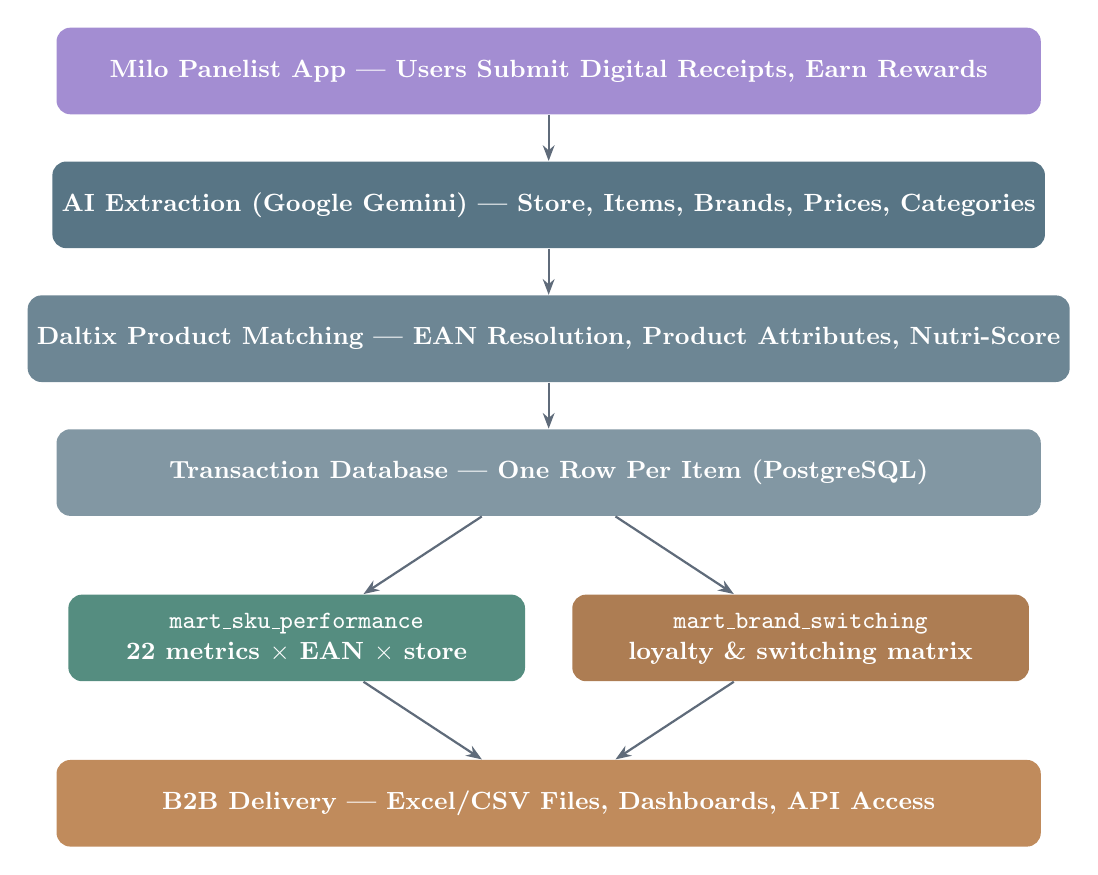
\begin{tikzpicture}[
  layer/.style={fill=#1, text=white, rounded corners=5pt, minimum width=12.5cm, minimum height=1.1cm, align=center, font=\small\bfseries},
  arrow/.style={-{Stealth[length=2mm]}, milogray, line width=0.8pt}
]
  \node[layer=milopurple!70] (app) at (0,0) {Milo Panelist App --- Users Submit Digital Receipts, Earn Rewards};
  \node[layer=miloprimary!80] (ai) at (0,-1.7) {AI Extraction (Google Gemini) --- Store, Items, Brands, Prices, Categories};
  \node[layer=miloprimary!70] (daltix) at (0,-3.4) {Daltix Product Matching --- EAN Resolution, Product Attributes, Nutri-Score};
  \node[layer=miloprimary!60] (db) at (0,-5.1) {Transaction Database --- One Row Per Item (PostgreSQL)};
  \node[layer=miloaccent!80!black, minimum width=5.8cm] (mart1) at (-3.2,-7.2) {\begin{tabular}{c}\texttt{mart\_sku\_performance}\\22 metrics $\times$ EAN $\times$ store\end{tabular}};
  \node[layer=milowarm!90!black, minimum width=5.8cm] (mart2) at (3.2,-7.2) {\begin{tabular}{c}\texttt{mart\_brand\_switching}\\loyalty \& switching matrix\end{tabular}};
  \node[layer=milowarm] (deliver) at (0,-9.3) {B2B Delivery --- Excel/CSV Files, Dashboards, API Access};

  \draw[arrow] (app) -- (ai);
  \draw[arrow] (ai) -- (daltix);
  \draw[arrow] (daltix) -- (db);
  \draw[arrow] (db) -- (mart1);
  \draw[arrow] (db) -- (mart2);
  \draw[arrow] (mart1) -- (deliver);
  \draw[arrow] (mart2) -- (deliver);
\end{tikzpicture}
\end{center}

\subsection{Data Product 1: \texttt{mart\_sku\_performance} (The Core Product)}

\begin{categorybox}
The core data product. Grain: \textbf{year\_month $\times$ EAN $\times$ store\_name}. Clients open this in Excel and pivot/filter using the included dimension attributes. Only includes Daltix-matched transactions (\texttt{ean IS NOT NULL}).

\vspace{0.5em}
\textbf{22 metrics across 6 categories:}

\vspace{0.5em}
\renewcommand{\arraystretch}{1.3}
\begin{tabularx}{\textwidth}{L{2.5cm} L{10.5cm}}
\toprule
\rowcolor{tabheader}
\textbf{\color{white}Category} & \textbf{\color{white}Metrics} \\
\midrule
\textbf{Shopper} & unique\_buyers, panel\_size, penetration\_pct, purchase\_frequency, avg\_basket\_spend, repeat\_buyer\_pct \\
\rowcolor{tabrow}
\textbf{Volume} & total\_spend, total\_units, avg\_spend\_per\_buyer \\
\textbf{Share} & category\_share\_pct, brand\_share\_in\_store\_pct, sku\_share\_of\_brand\_pct \\
\rowcolor{tabrow}
\textbf{Pricing} & avg\_paid\_price, avg\_shelf\_price, price\_gap\_pct, avg\_price\_per\_volume \\
\textbf{Promo} & promo\_share\_pct, avg\_promo\_depth\_pct, promo\_volume\_uplift, promo\_types \\
\rowcolor{tabrow}
\textbf{Quality} & total\_transactions, avg\_match\_confidence \\
\bottomrule
\end{tabularx}

\vspace{0.5em}
\textbf{Dimension attributes included for pivoting:} product\_name, brand\_name, manufacturer, is\_private\_label, granular\_category, parent\_category, group\_name, pack\_size, pack\_unit, nutri\_score, retailer\_group, store\_type, is\_discounter.

\vspace{0.3em}
{\small\color{milogray} For hard discounters, \texttt{sku\_resolution\_type = `representative'} rows use a representative EAN with \texttt{represented\_eans} showing all possible variants.}
\end{categorybox}

\subsection{Data Product 2: \texttt{mart\_brand\_switching} (Brand Loyalty \& Switching Matrix)}

\begin{categorybox}
A brand-to-brand transition matrix tracking how consumers move between brands within each category. Grain: \textbf{year\_month $\times$ granular\_category $\times$ from\_brand $\times$ to\_brand}.

\vspace{0.3em}
{\small Reading the matrix: row = from\_brand, column = to\_brand. Diagonal = loyalty (repeat buyers). Off-diagonal = switching (brand changers).}

\vspace{0.5em}
\renewcommand{\arraystretch}{1.3}
\begin{tabularx}{\textwidth}{L{2.8cm} L{10.2cm}}
\toprule
\rowcolor{tabheader}
\textbf{\color{white}Category} & \textbf{\color{white}Metrics} \\
\midrule
\textbf{Switching} & switcher\_count, total\_switches, switch\_share\_pct, reverse\_switch\_count, net\_flow \\
\rowcolor{tabrow}
\textbf{Loyalty} & loyalty\_rate\_pct, avg\_days\_between\_repeat \\
\textbf{Cannibalization} & intra\_brand\_switch\_count, intra\_brand\_switch\_pct \\
\rowcolor{tabrow}
\textbf{Value} & avg\_from\_price, avg\_to\_price, price\_direction, switched\_spend \\
\textbf{Promo} & promo\_driven\_switch\_pct, post\_promo\_retention\_pct \\
\bottomrule
\end{tabularx}
\end{categorybox}

\subsection{What Makes Milo Data Unique}

\begin{enumerate}[leftmargin=1.5em, itemsep=3pt]
  \item \textbf{SKU-level granularity via Daltix matching} --- actual EAN codes, not just brand-level. Enables pack-size analysis, variant comparison, and true product-level performance tracking.
  \item \textbf{Actual prices paid} --- not shelf prices. What consumers actually paid, including discounts and promotions. The \texttt{price\_gap\_pct} metric quantifies the gap.
  \item \textbf{Cross-retailer promo tracking} --- promo\_share\_pct, promo\_depth, and promo\_volume\_uplift show exactly how promotions perform across different retailers.
  \item \textbf{Brand switching intelligence} --- the only affordable source of brand-to-brand switching data in Belgium. Shows where consumers go when they leave your brand, and why.
  \item \textbf{Full-basket context} --- what's bought together reveals basket affinity and cross-purchase patterns.
  \item \textbf{High-quality panel} --- Milo users submit frequently because they genuinely use the app, not just for minimal rewards. Quality is tracked via \texttt{avg\_match\_confidence}.
\end{enumerate}

\subsection{Example: What the Data Answers}

\begin{qabox}
\textbf{A Belgian beer brand director asks: ``Are we losing share to private label?''}\\[4pt]
{\small\color{milogray} \textbf{From \texttt{mart\_sku\_performance}:} Based on our panel of 5,000 Belgian households: \textbf{Yes, but only at Aldi.} Jupiler holds 38\% value share at Colruyt (stable), 34\% at Delhaize (stable), but dropped from 22\% to 16\% at Aldi. Cara Pils grew from 31\% to 39\% at Aldi in the same period. The shift is price-driven: avg\_paid\_price for Jupiler at Aldi is \texteuro{}14.99/crate vs.\ Cara Pils at \texteuro{}9.99.}
\end{qabox}

\vspace{0.3em}

\begin{qabox}
\textbf{The same beer brand director asks: ``Where are my lost customers going?''}\\[4pt]
{\small\color{milogray} \textbf{From \texttt{mart\_brand\_switching}:} In the Beer Pils category at Aldi, the Jupiler $\rightarrow$ Cara Pils row shows: switcher\_count = 340, switch\_share\_pct = 62\%, promo\_driven\_switch\_pct = 78\%. But post\_promo\_retention\_pct is only 23\% --- meaning most switchers return after the promo ends. \textbf{Recommendation:} The switching is promo-driven and largely temporary. Focus on matching promo timing rather than permanent price cuts.}
\end{qabox}

\vspace{0.3em}

\begin{qabox}
\textbf{An SMB pasta sauce maker asks: ``I want to get listed at Colruyt. What should I know?''}\\[4pt]
{\small\color{milogray} \textbf{From \texttt{mart\_sku\_performance}:} Premium pasta sauce ({>}\texteuro{}3.50/jar) has a penetration\_pct of 14\% at Colruyt --- but growing +2pt/quarter. Private label holds category\_share\_pct of 39\%, Barilla 21\%. There's a gap for a Belgian artisanal brand at \texteuro{}4--5. The avg\_promo\_depth\_pct for the category is 18\%, suggesting moderate promo activity. Without our data, this producer walks into Colruyt with nothing but a product sample and hope.}
\end{qabox}

\clearpage

% ============================================================================
% 7. CATEGORY DATA SUBSCRIPTIONS
% ============================================================================
\section{Category Data Subscriptions}

\subsection{How It Works}

Clients subscribe to the \textbf{product categories they compete in}, choose their \textbf{data depth tier}, and select which \textbf{data products} they need:

\begin{center}
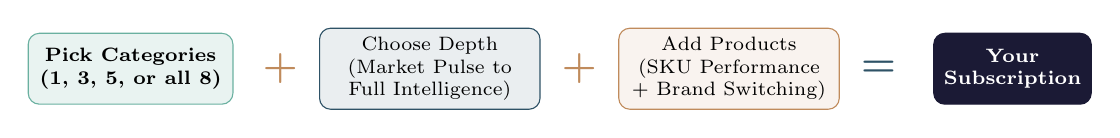
\begin{tikzpicture}[
  catbox/.style={fill=miloaccent!15, draw=miloaccent, rounded corners=4pt, minimum width=2.6cm, minimum height=0.9cm, align=center, font=\scriptsize\bfseries},
  tierbox/.style={fill=miloprimary!10, draw=miloprimary, rounded corners=4pt, minimum width=2.8cm, minimum height=0.9cm, align=center, font=\scriptsize},
  prodbox/.style={fill=milowarm!10, draw=milowarm, rounded corners=4pt, minimum width=2.8cm, minimum height=0.9cm, align=center, font=\scriptsize},
  plusnode/.style={font=\Large\bfseries\color{milowarm}},
  eqnode/.style={font=\Large\bfseries\color{miloprimary}}
]
  \node[catbox] (cat) at (0,0) {Pick Categories\\(1, 3, 5, or all 8)};
  \node[plusnode] at (1.9,0) {+};
  \node[tierbox] (tier) at (3.8,0) {Choose Depth\\(Market Pulse to\\Full Intelligence)};
  \node[plusnode] at (5.7,0) {+};
  \node[prodbox] (prod) at (7.6,0) {Add Products\\(SKU Performance\\+ Brand Switching)};
  \node[eqnode] at (9.5,0) {=};
  \node[catbox, fill=milodark, text=white, draw=milodark, minimum width=2cm] (result) at (11.2,0) {Your\\Subscription};
\end{tikzpicture}
\end{center}

\subsection{Eight Category Domains}

\begin{center}
\renewcommand{\arraystretch}{1.35}
\begin{tabularx}{\textwidth}{C{0.6cm} L{3.8cm} L{5cm} R{1.5cm} R{2.5cm}}
\toprule
\rowcolor{tabheader}
\textbf{\color{white}\#} & \textbf{\color{white}Category Domain} & \textbf{\color{white}Includes} & \textbf{\color{white}Granular Cat.} & \textbf{\color{white}Potential Clients} \\
\midrule
1 & Dairy, Eggs \& Cheese & Yoghurt, Milk, Cheese, Butter, Eggs, Cream & $\sim$30 & 320+ \\
\rowcolor{tabrow}
2 & Bakery \& Cereals & Bread, Pastry, Cereals, Muesli, Baking & $\sim$25 & 280+ \\
3 & Meat, Fish \& Deli & Fresh meat, Charcuterie, Fish, Plant-based & $\sim$20 & 220+ \\
\rowcolor{tabrow}
4 & Beverages & Beer, Wine, Spirits, Soft Drinks, Coffee, Tea & $\sim$35 & 580+ \\
5 & Pantry \& Cooking & Sauces, Pasta, Rice, Oils, Condiments, Spices & $\sim$30 & 450+ \\
\rowcolor{tabrow}
6 & Snacks \& Confectionery & Chocolate, Chips, Biscuits, Candy, Nuts & $\sim$25 & 380+ \\
7 & Frozen \& Ready Meals & Frozen meals, Frozen veg, Pizza, Ice cream & $\sim$15 & 180+ \\
\rowcolor{tabrow}
8 & Household \& Personal Care & Cleaning, Detergent, Skincare, Pet Food & $\sim$20 & 220+ \\
\midrule
& \textbf{Full Market Access} & \textbf{All 8 category domains combined} & \textbf{$\sim$200} & \textbf{3,900+} \\
\bottomrule
\end{tabularx}
\end{center}

\subsection{Four Data Depth Tiers}

\begin{center}
\renewcommand{\arraystretch}{1.4}
\begin{tabularx}{\textwidth}{L{2.8cm} R{2cm} L{8.5cm}}
\toprule
\rowcolor{tabheader}
\textbf{\color{white}Depth Tier} & \textbf{\color{white}Per Category} & \textbf{\color{white}What You Get} \\
\midrule
\textbf{Market Pulse} & \texteuro{}149/mo & Top-line metrics from \texttt{mart\_sku\_performance} across all retailers combined. Category size, penetration, growth trends, top brands, private label share. \\
\rowcolor{tabrow}
\textbf{Retailer View} & \texteuro{}299/mo & Everything in Market Pulse, broken down by retailer and store. Full SKU-level granularity with all 22 metrics per EAN $\times$ store. \\
\textbf{Brand Intelligence} & \texteuro{}499/mo & Retailer View + \texttt{mart\_brand\_switching}: brand-to-brand transition matrix, loyalty rates, promo-driven switching, net flow analysis. \\
\rowcolor{tabrow}
\textbf{Full Intelligence} & \texteuro{}799/mo & Everything above + private label deep-dive, pricing analytics (price\_gap\_pct, promo\_depth), demographic breakdowns, cross-purchase patterns. \\
\bottomrule
\end{tabularx}
\end{center}

\subsection{Bundle Pricing}

\begin{center}
\renewcommand{\arraystretch}{1.4}
\begin{tabularx}{\textwidth}{L{3cm} C{2cm} R{2.5cm} R{2.5cm} L{3cm}}
\toprule
\rowcolor{tabheader}
\textbf{\color{white}Bundle} & \textbf{\color{white}Discount} & \textbf{\color{white}Market Pulse} & \textbf{\color{white}Full Intelligence} & \textbf{\color{white}Ideal For} \\
\midrule
Single Category & --- & \texteuro{}149/mo & \texteuro{}799/mo & SMB brands \\
\rowcolor{tabrow}
3 Categories & 15\% off & \texteuro{}380/mo & \texteuro{}2,037/mo & Mid-size brands \\
5 Categories & 25\% off & \texteuro{}559/mo & \texteuro{}2,996/mo & Diversified producers \\
\rowcolor{tabrow}
Full Market (8) & 40\% off & \texteuro{}715/mo & \texteuro{}3,835/mo & Retailers \& agencies \\
\bottomrule
\end{tabularx}
\end{center}

\begin{alertbox}
\textbf{Key insight:} A small Belgian cheese maker can access SKU-level cross-retailer dairy intelligence for \texteuro{}127/month (annual Market Pulse) --- including actual EAN performance, pricing analytics, and promo effectiveness. Previously, the minimum entry point for any cross-retailer data was \texteuro{}100,000+/year.\textsuperscript{[3]} We reduce the barrier by \textbf{98.5\%}.
\end{alertbox}

\clearpage

% ============================================================================
% 8. TARGET CLIENTS & MARKET REACH
% ============================================================================
\section{Target Clients \& Market Reach}

\subsection{Client Summary}

\begin{center}
\renewcommand{\arraystretch}{1.35}
\begin{tabularx}{\textwidth}{L{4cm} R{2cm} R{2cm} R{2cm} R{2cm}}
\toprule
\rowcolor{tabheader}
\textbf{\color{white}Category Domain} & \textbf{\color{white}SMBs} & \textbf{\color{white}Mid-Size} & \textbf{\color{white}Enterprise} & \textbf{\color{white}Total} \\
\midrule
Dairy, Eggs \& Cheese & 250 & 50 & 20 & 320 \\
\rowcolor{tabrow}
Bakery \& Cereals & 200 & 55 & 25 & 280 \\
Meat, Fish \& Deli & 155 & 45 & 20 & 220 \\
\rowcolor{tabrow}
Beverages & 430 & 100 & 50 & 580 \\
Pantry \& Cooking & 320 & 90 & 40 & 450 \\
\rowcolor{tabrow}
Snacks \& Confectionery & 275 & 70 & 35 & 380 \\
Frozen \& Ready Meals & 110 & 45 & 25 & 180 \\
\rowcolor{tabrow}
Household \& Personal Care & 140 & 50 & 30 & 220 \\
\midrule
\textbf{Total} & \textbf{1,880} & \textbf{505} & \textbf{245} & \textbf{2,630} \\
\midrule
\rowcolor{tabrow}
Cross-category + agencies + retail & --- & 180 & 95 & 275 \\
\midrule
\textbf{Grand Total (unique)} & & & & \textbf{3,900+} \\
\bottomrule
\end{tabularx}
\end{center}

\subsection{Named Target Clients}

\begin{productbox}
\textbf{\color{miloprimary}Enterprise Targets (\texteuro{}2,000--8,000/mo)}\\[4pt]
\begin{multicols}{3}
\begin{itemize}[leftmargin=1em, itemsep=1pt, font=\small]
  \item AB InBev Belgium
  \item Danone Belgium
  \item Coca-Cola Europacific
  \item Nestl\'{e} Belgium
  \item Mondelez / C\^{o}te d'Or
  \item Procter \& Gamble
  \item Unilever Belgium
  \item Colruyt Group (PL)
  \item Delhaize (commercial)
  \item Lotus Bakeries
  \item FrieslandCampina
  \item Henkel Belgium
\end{itemize}
\end{multicols}
\end{productbox}

\begin{productbox}
\textbf{\color{miloprimary}Mid-Size Targets (\texteuro{}500--2,000/mo)}\\[4pt]
\begin{multicols}{3}
\begin{itemize}[leftmargin=1em, itemsep=1pt, font=\small]
  \item Devos-Lemmens
  \item La William
  \item Imperial Meat Products
  \item Duvel-Moortgat
  \item Alken-Maes
  \item Ter Beke
  \item Vandermoortele
  \item Spadel / Bru
  \item Ecover
  \item Leonidas
  \item Milcobel
  \item Greenyard
\end{itemize}
\end{multicols}
\end{productbox}

\begin{productbox}
\textbf{\color{miloprimary}SMB Targets --- \texteuro{}149--499/mo (the underserved majority)}\\[4pt]
\begin{multicols}{3}
\begin{itemize}[leftmargin=1em, itemsep=1pt, font=\small]
  \item 350+ craft breweries
  \item 150+ cheese makers
  \item 120+ chocolate producers
  \item 80+ sauce producers
  \item 60+ meat processors
  \item 50+ biscuit brands
  \item 40+ organic startups
  \item 35+ coffee roasters
  \item Plant-based brands
\end{itemize}
\end{multicols}
\end{productbox}

\clearpage

% ============================================================================
% 9. COMPETITIVE LANDSCAPE
% ============================================================================
\section{Competitive Landscape}

\subsection{The Structural Gap}

\begin{center}
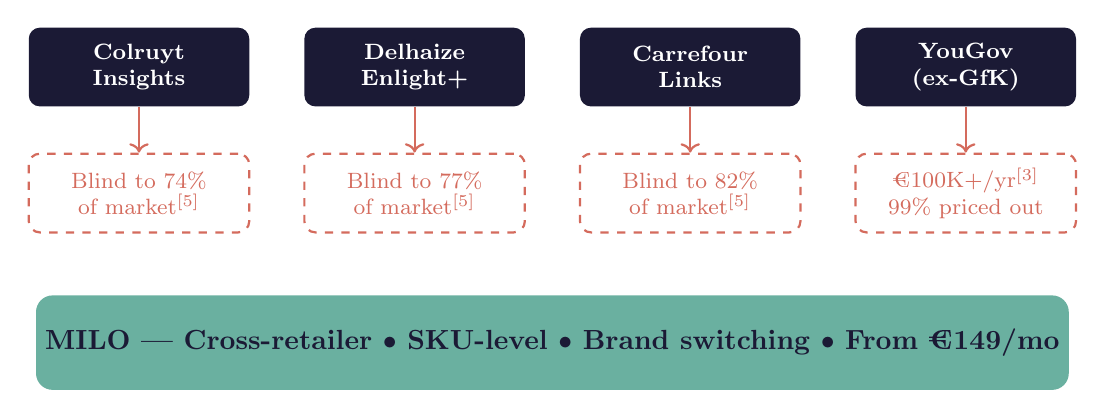
\begin{tikzpicture}[
  every node/.style={font=\footnotesize},
  retailer/.style={fill=milodark, text=white, rounded corners=4pt, minimum width=2.8cm, minimum height=1cm, align=center, font=\footnotesize\bfseries},
  blind/.style={draw=milored, dashed, thick, rounded corners=4pt, minimum width=2.8cm, minimum height=1cm, align=center, font=\footnotesize\color{milored}},
  milo/.style={fill=miloaccent, text=milodark, rounded corners=6pt, minimum width=12cm, minimum height=1.2cm, align=center, font=\normalsize\bfseries}
]
  \node[retailer] (col) at (0,0) {Colruyt\\Insights};
  \node[retailer] (del) at (3.5,0) {Delhaize\\Enlight+};
  \node[retailer] (car) at (7,0) {Carrefour\\Links};
  \node[retailer] (you) at (10.5,0) {YouGov\\(ex-GfK)};

  \node[blind] (colb) at (0,-1.6) {Blind to 74\%\\of market\textsuperscript{[5]}};
  \node[blind] (delb) at (3.5,-1.6) {Blind to 77\%\\of market\textsuperscript{[5]}};
  \node[blind] (carb) at (7,-1.6) {Blind to 82\%\\of market\textsuperscript{[5]}};
  \node[blind] (youb) at (10.5,-1.6) {\texteuro{}100K+/yr\textsuperscript{[3]}\\99\% priced out};

  \draw[->, milored, thick] (col) -- (colb);
  \draw[->, milored, thick] (del) -- (delb);
  \draw[->, milored, thick] (car) -- (carb);
  \draw[->, milored, thick] (you) -- (youb);

  \node[milo] at (5.25,-3.5) {MILO --- Cross-retailer $\bullet$ SKU-level $\bullet$ Brand switching $\bullet$ From \texteuro{}149/mo};
\end{tikzpicture}
\end{center}

\subsection{Panelist App Competitive Advantages}

\begin{center}
\renewcommand{\arraystretch}{1.3}
\begin{tabularx}{\textwidth}{L{3cm} C{1.8cm} C{1.8cm} C{2cm} C{1.8cm} C{1.8cm}}
\toprule
\rowcolor{tabheader}
\textbf{\color{white}Feature} & \textbf{\color{white}Milo} & \textbf{\color{white}Bankin'} & \textbf{\color{white}Cake (BNP)} & \textbf{\color{white}Toshl} & \textbf{\color{white}Shopmium} \\
\midrule
Item-level data & \textbf{\color{milogreen}Yes} & \textcolor{milored}{No} & \textcolor{milored}{No} & \textcolor{milored}{No} & Partial \\
\rowcolor{tabrow}
Health scoring & \textbf{\color{milogreen}Yes} & \textcolor{milored}{No} & \textcolor{milored}{No} & \textcolor{milored}{No} & \textcolor{milored}{No} \\
AI assistant & \textbf{\color{milogreen}Yes} & \textcolor{milored}{No} & \textcolor{milored}{No} & \textcolor{milored}{No} & \textcolor{milored}{No} \\
\rowcolor{tabrow}
Cash rewards & \textbf{\color{milogreen}\texteuro{}0.50+} & \textcolor{milored}{No} & \textcolor{milored}{No} & \textcolor{milored}{No} & Per product \\
Deals engine & \textbf{\color{milogreen}Yes} & \textcolor{milored}{No} & \textcolor{milored}{No} & \textcolor{milored}{No} & Yes \\
\rowcolor{tabrow}
BE grocery focus & \textbf{\color{milogreen}13 stores} & Generic & \textcolor{milored}{No} & Generic & Partial \\
\bottomrule
\end{tabularx}
\end{center}

\subsection{Milo vs PROMOS: B2C App Comparison}

The closest structural parallel to Milo's B2C app is \textbf{PROMOS} --- the consumer cashback app operated by Promos Cupones Digitales S.L. in Spain (the B2C front-end of Algori). A detailed comparison reveals Milo's structural advantages on every key dimension:\textsuperscript{[23][27][28]}

\begin{center}
\renewcommand{\arraystretch}{1.35}
\begin{tabularx}{\textwidth}{L{3.2cm} L{5.1cm} L{5.1cm}}
\toprule
\rowcolor{tabheader}
\textbf{\color{white}Dimension} & \textbf{\color{white}PROMOS (Algori) --- Spain} & \textbf{\color{white}Milo --- Belgium} \\
\midrule
Panel size & $\sim$45,000 weekly active\textsuperscript{[23]} & Pre-launch; targeting 500 $\rightarrow$ 5K $\rightarrow$ 30K \\
\rowcolor{tabrow}
Total funding & \texteuro{}7.5M+\textsuperscript{[23]} & Seeking \texteuro{}150K--250K seed \\
Receipt type & Camera photos (OCR)\textsuperscript{[27]} & Digital receipts only (pre-structured) \\
\rowcolor{tabrow}
Base reward/receipt & \texteuro{}0.00 (no base reward)\textsuperscript{[27][28]} & \texteuro{}0.50--0.75 (guaranteed) \\
Gamification & None\textsuperscript{[27]} & 4-tier with spins, streaks, jackpots \\
\rowcolor{tabrow}
App utility & None beyond cashback\textsuperscript{[27]} & Spending analytics, health scoring, AI chat \\
Data enrichment & Receipt text only & Daltix EAN + shelf prices + promo data \\
\rowcolor{tabrow}
Product matching & Internal AI classification & Daltix EAN resolution + Nutri-Score \\
Promo tracking & Cannot determine if on promo\textsuperscript{[27]} & Yes (via Daltix shelf data) \\
\rowcolor{tabrow}
Price analysis & No price gap metric & price\_gap\_pct (actual vs shelf) \\
B2B pricing & Custom enterprise only\textsuperscript{[23]} & Per-category from \texteuro{}149/mo \\
\rowcolor{tabrow}
User sentiment & 1.6/5 Trustpilot\textsuperscript{[28]} & Not yet live \\
\bottomrule
\end{tabularx}
\end{center}

\vspace{0.5em}

\subsubsection{Five Structural Advantages of Milo Over PROMOS}

\begin{enumerate}[leftmargin=1.5em, itemsep=6pt]

  \item \textbf{Data quality --- digital receipts + Daltix enrichment beats camera OCR.}
  PROMOS requires users to photograph physical receipts, which introduces OCR errors, image quality issues, and incomplete captures.\textsuperscript{[27]} Milo accepts only digital receipts (email receipts, PDF receipts, e-receipts), which arrive as pre-structured text --- eliminating OCR errors entirely. More importantly, every Milo transaction is enriched via Daltix with exact EAN codes, Nutri-Score, shelf prices, and promotion flags. PROMOS has no equivalent enrichment layer, meaning it cannot compute Milo's most distinctive metrics: \texttt{price\_gap\_pct}, promo effectiveness, or Nutri-Score-weighted health analytics.

  \item \textbf{Complete basket capture --- spend-based rewards capture ALL trips, not just promo-relevant ones.}
  PROMOS rewards users only when specific promoted products appear on a receipt.\textsuperscript{[27]} This creates a structurally biased panel: users only submit receipts when they happen to have bought a promoted product. Entire shopping trips are missed. Milo pays \texteuro{}0.50+ per receipt regardless of content, creating an incentive to submit every grocery trip. For B2B clients, this difference is critical --- Milo captures full baskets, full purchase missions, and full price histories rather than promo-biased snapshots.

  \item \textbf{Consumer app as a product --- five retention moats vs.\ bare-bones data collection.}
  PROMOS has no standalone utility beyond cashback.\textsuperscript{[27]} Its 1.6/5 Trustpilot rating\textsuperscript{[28]} reflects complaints about shrinking rewards (from \texteuro{}0.10 to \texteuro{}0.01 per promo), opaque rejection processes, and zero reasons to return beyond checking for new promos. Milo is designed to be genuinely useful as a personal finance and health tool --- spending analytics, AI chat, health scoring, deal recommendations, expense splitting, and a loyalty card wallet. The five retention moats (wallet balance, streaks, badges, purchase history, AI context) create a product that users return to daily, not just when they remember to scan a receipt.

  \item \textbf{Belgium market concentration --- 5 retailers = 85\%+ coverage (easier than Spain's fragmented market).}
  Spain's grocery retail market is structurally fragmented: 15+ major chains, strong regional players, and significant independent retail.\textsuperscript{[5][23]} Belgium's market is the opposite: five retailers (Colruyt Group, Ahold Delhaize, Carrefour, Lidl, Aldi) control over 85\% of grocery sales.\textsuperscript{[5]} This means Milo can achieve near-complete market coverage with a panel that is proportionally much smaller than what Algori requires in Spain. The structural economics of the Belgian market make Milo's path to data completeness faster and cheaper per panelist.

  \item \textbf{Promo effectiveness measurement --- combining receipt data with Daltix promo data is the holy grail for FMCG trade marketing.}
  The single most valuable insight for a Belgian FMCG brand manager is whether their trade promotions are driving incremental volume or merely subsidizing existing buyers. PROMOS cannot answer this: without shelf price data, it is impossible to determine whether any given purchase was made at a promotional price.\textsuperscript{[27]} Milo's Daltix integration provides real-time shelf and promotion data for every SKU at every retailer. By comparing \texttt{avg\_paid\_price} against \texttt{avg\_shelf\_price}, Milo produces \texttt{price\_gap\_pct} and \texttt{promo\_share\_pct} --- metrics that directly measure promotional uptake and trade spend efficiency. This is data that FMCG brands currently pay premium-priced consultants to approximate from incomplete sources.

\end{enumerate}

\subsection{12 Competitive Advantages (Combined)}

\begin{enumerate}[leftmargin=1.5em, itemsep=3pt]
  \item \textbf{Free panelist app:} Zero cost to the user eliminates adoption friction. B2B data revenue funds the entire operation.
  \item \textbf{Cross-retailer view:} Colruyt, Delhaize, Carrefour, Lidl, Aldi --- all in one dataset. Retailers will \emph{never} share this with each other.
  \item \textbf{SKU-level via Daltix matching:} Real EAN codes, not just brand-level. Enables pack-size and variant analysis that brand-level panels cannot provide.
  \item \textbf{Brand switching matrix:} The only affordable source of brand-to-brand transition data in Belgium --- loyalty rates, promo-driven switching, net flow.
  \item \textbf{Per-category pricing:} No competitor offers modular, per-category subscriptions. All-or-nothing everywhere else.
  \item \textbf{Actual prices paid:} Not shelf prices --- what consumers actually handed over, including discounts. The \texttt{price\_gap\_pct} metric quantifies the difference.
  \item \textbf{AI-powered insights:} Both consumer-facing (Milo chat) and B2B-facing (analytics dashboards).
  \item \textbf{Belgium-specific depth:} 13 store chains, 3 languages, Belgian grocery taxonomy. The specialist advantage.
  \item \textbf{SMB-accessible:} 10--100$\times$ cheaper than YouGov/GfK for the most-valued KPIs.\textsuperscript{[3]}
  \item \textbf{Compounding data moat:} Historical data becomes more valuable every month. First-mover advantage in cross-retailer data.
\end{enumerate}

\subsection{Comparable Companies}

\begin{center}
\renewcommand{\arraystretch}{1.3}
\begin{tabularx}{\textwidth}{L{3cm} L{2.8cm} R{2.5cm} L{4.5cm}}
\toprule
\rowcolor{tabheader}
\textbf{\color{white}Company} & \textbf{\color{white}Model} & \textbf{\color{white}Scale} & \textbf{\color{white}Key Insight for Milo} \\
\midrule
Fetch Rewards (US) & Receipt rewards + data & \$2.5B+ valuation\textsuperscript{[10]} & 11M receipts/day proves the model \\
\rowcolor{tabrow}
Ibotta (US) & Receipt rewards + data & \$367M rev (2024)\textsuperscript{[11]} & Publicly traded (IPO Apr 2024); audience segments \\
Foxintelligence (FR) & E-receipt panel & Acquired by NIQ\textsuperscript{[12]} & EU receipt data proven valuable \\
\rowcolor{tabrow}
Shopmium (FR/BE) & Cashback + data & 10M+ downloads\textsuperscript{[13]} & Nielsen partnership; biased panel \\
NielsenIQ Byzzer (US) & SMB data platform & Part of \$3.5B NIQ\textsuperscript{[14]} & US-only; no EU equivalent exists \\
\rowcolor{tabrow}
\textbf{Algori (ES)}\textsuperscript{[23]} & Receipt panel + AI analytics & \texteuro{}7.5M funding / 45K panelists & Proved model works; Milo's B2C app is structurally stronger \\
\bottomrule
\end{tabularx}
\end{center}

\clearpage

% ============================================================================
% 10. TECHNOLOGY & ARCHITECTURE
% ============================================================================
\section{Technology \& Architecture}

\subsection{Technical Stack}

\begin{center}
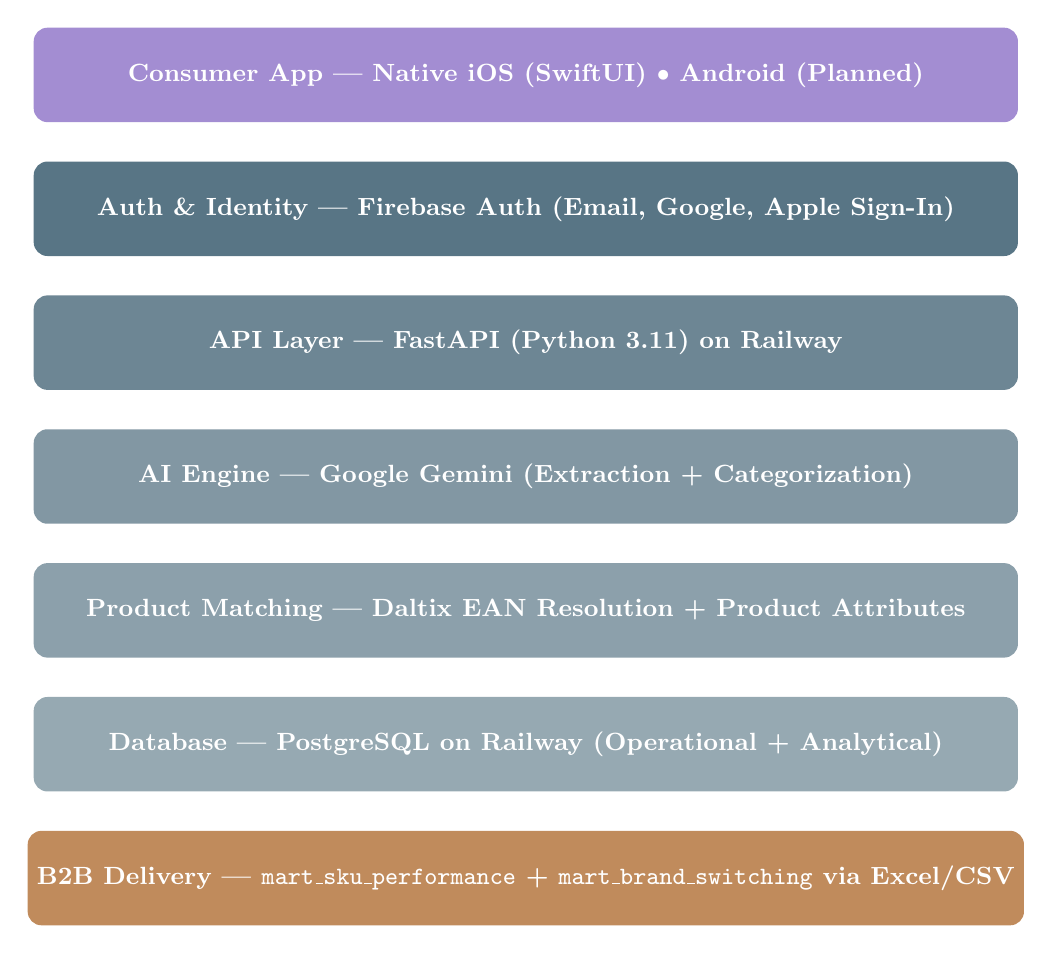
\begin{tikzpicture}[
  layer/.style={fill=#1, text=white, rounded corners=5pt, minimum width=12.5cm, minimum height=1.2cm, align=center, font=\small\bfseries}
]
  \node[layer=milopurple!70] (app) at (0,0) {Consumer App --- Native iOS (SwiftUI) $\bullet$ Android (Planned)};
  \node[layer=miloprimary!80] (auth) at (0,-1.7) {Auth \& Identity --- Firebase Auth (Email, Google, Apple Sign-In)};
  \node[layer=miloprimary!70] (api) at (0,-3.4) {API Layer --- FastAPI (Python 3.11) on Railway};
  \node[layer=miloprimary!60] (ai) at (0,-5.1) {AI Engine --- Google Gemini (Extraction + Categorization)};
  \node[layer=miloprimary!55] (daltix) at (0,-6.8) {Product Matching --- Daltix EAN Resolution + Product Attributes};
  \node[layer=miloprimary!50] (db) at (0,-8.5) {Database --- PostgreSQL on Railway (Operational + Analytical)};
  \node[layer=milowarm] (delivery) at (0,-10.2) {B2B Delivery --- \texttt{mart\_sku\_performance} + \texttt{mart\_brand\_switching} via Excel/CSV};
\end{tikzpicture}
\end{center}

\subsection{iOS App Architecture}

\begin{center}
\renewcommand{\arraystretch}{1.3}
\begin{tabularx}{\textwidth}{L{3.5cm} L{10cm}}
\toprule
\rowcolor{tabheader}
\textbf{\color{white}Component} & \textbf{\color{white}Technology} \\
\midrule
Framework & SwiftUI with MVVM architecture \\
\rowcolor{tabrow}
Concurrency & @MainActor ViewModels, Actor-based services for thread safety \\
Share Extension & App Group data sharing for receipt import from any app \\
\rowcolor{tabrow}
Caching & Disk-backed caching --- 12 months of data cached locally \\
Preloading & Multi-phase data preloading on app launch (4 parallel phases) \\
\rowcolor{tabrow}
In-App Purchases & StoreKit 2 integration (ready for future coupon marketplace) \\
\rowcolor{tabrow}
Wallet & PassKit for Apple Wallet loyalty card integration \\
AI Chat & SSE streaming for real-time Milo responses \\
\rowcolor{tabrow}
Animations & Spring physics, 3D card flips, confetti particles, haptic feedback \\
\bottomrule
\end{tabularx}
\end{center}

\subsection{Backend Architecture}

\begin{center}
\renewcommand{\arraystretch}{1.3}
\begin{tabularx}{\textwidth}{L{3.5cm} L{10cm}}
\toprule
\rowcolor{tabheader}
\textbf{\color{white}Component} & \textbf{\color{white}Technology} \\
\midrule
API Framework & FastAPI (Python 3.11) with async endpoints \\
\rowcolor{tabrow}
Hosting & Railway with separate non-prod and production environments \\
Database & PostgreSQL with Alembic migrations \\
\rowcolor{tabrow}
AI/ML Pipeline & Google Gemini for extraction $\rightarrow$ categorization $\rightarrow$ health scoring \\
Product Matching & Daltix integration for EAN resolution + product attributes (Nutri-Score, pack size, manufacturer) \\
\rowcolor{tabrow}
Promo Matching & Pinecone vector search for deal personalization \\
Auth & Firebase Auth token verification \\
\bottomrule
\end{tabularx}
\end{center}

\subsection{GDPR Compliance}

\begin{itemize}[leftmargin=1.5em, itemsep=3pt]
  \item \textbf{Explicit consent:} Users opt-in to data collection and anonymized data sharing during onboarding
  \item \textbf{Anonymization:} All B2B data products use aggregated, anonymized data. Minimum group sizes of 30--50 per reported cell
  \item \textbf{Right to erasure:} Users can delete all their data at any time
  \item \textbf{DPA compliance:} Aligned with Belgian Data Protection Authority (APD/GBA) requirements
  \item \textbf{Data Processing Agreements:} All B2B clients sign DPAs prohibiting re-identification
\end{itemize}

\clearpage

% ============================================================================
% 11. GO-TO-MARKET STRATEGY
% ============================================================================
\section{Go-to-Market Strategy}

\subsection{Panelist Acquisition (Milo App)}

\begin{center}
\renewcommand{\arraystretch}{1.3}
\begin{tabularx}{\textwidth}{C{2cm} C{2cm} L{9cm}}
\toprule
\rowcolor{tabheader}
\textbf{\color{white}Phase} & \textbf{\color{white}Users} & \textbf{\color{white}Strategy} \\
\midrule
Months 1--2 & 0--500 & Friends \& family, social media launch, Belgian food/finance influencers. All users get premium free. \\
\rowcolor{tabrow}
Months 3--4 & 500--2K & Paid social (Instagram, TikTok targeting Belgian grocery shoppers), university partnerships, referral program (invite $\rightarrow$ bonus spins) \\
Months 5--8 & 2K--5K & App Store Optimization, PR in Belgian media (De Tijd, HLN), Flemish \& Walloon content marketing \\
\rowcolor{tabrow}
Months 9--12 & 5K--10K & Organic growth from word-of-mouth, loyalty program maturity, first viral moments from jackpot winners \\
Year 2 & 10K--30K & Multi-channel paid + organic. Android launch doubles addressable market. Referral flywheel. \\
\bottomrule
\end{tabularx}
\end{center}

\subsection{B2B Sales (Data Subscriptions)}

\begin{center}
\renewcommand{\arraystretch}{1.3}
\begin{tabularx}{\textwidth}{C{2cm} C{2cm} L{9cm}}
\toprule
\rowcolor{tabheader}
\textbf{\color{white}Phase} & \textbf{\color{white}Clients} & \textbf{\color{white}Strategy} \\
\midrule
Months 5--6 & Leads & First sample category reports from real data. Outreach to 15--20 prospects per category. Free category snapshots as lead magnets. \\
\rowcolor{tabrow}
Months 7--9 & 5--8 & First paying subscribers. \texttt{mart\_sku\_performance} as core offering. Datarade listing for inbound leads. \\
Months 10--12 & 10--18 & Launch \texttt{mart\_brand\_switching} add-on. LinkedIn outreach to brand managers. Industry event presentations (Fevia, SIAL). \\
\rowcolor{tabrow}
Year 2 & 25--50 & Full product suite. Enterprise contracts. Analytics premium pilots. Pre-sales for Netherlands expansion. \\
Year 3 & 50--80 & Multi-category bundles driving ARPC up. Standard analytics offering. First cross-border data. \\
\bottomrule
\end{tabularx}
\end{center}

\subsection{Expansion Roadmap}

The app architecture already supports geographic expansion:

\begin{itemize}[leftmargin=1.5em, itemsep=3pt]
  \item \textbf{Netherlands} (Year 2--3): Albert Heijn and Jumbo already in the store list. Dutch language already supported. Natural bridge from Belgian operations.
  \item \textbf{France} (Year 3+): Carrefour and Intermarch\'{e} already supported. French language already built. Massive TAM.
  \item \textbf{Adding new markets requires:} Store database additions, AI training on new receipt formats, promotional data feeds. Core infrastructure is market-agnostic.
\end{itemize}

\clearpage

% ============================================================================
% 12. FINANCIAL PROJECTIONS
% ============================================================================
\section{Financial Projections}

\subsection{Cost Structure}

\begin{center}
\renewcommand{\arraystretch}{1.3}
\begin{tabularx}{\textwidth}{L{5cm} R{2.5cm} R{2.5cm} R{2.5cm}}
\toprule
\rowcolor{tabheader}
\textbf{\color{white}Cost Item} & \textbf{\color{white}Year 1} & \textbf{\color{white}Year 2} & \textbf{\color{white}Year 3} \\
\midrule
\multicolumn{4}{l}{\textbf{\color{milopurple!80}\small Panelist App Costs}} \\
\midrule
User rewards (wallet credits)\textsuperscript{1} & \texteuro{}15K--25K & \texteuro{}60K--100K & \texteuro{}150K--250K \\
\rowcolor{tabrow}
Coupon redemptions (net)\textsuperscript{2} & \texteuro{}8K--15K & \texteuro{}30K--55K & \texteuro{}70K--130K \\
User acquisition (ads, referrals) & \texteuro{}25K--50K & \texteuro{}30K--50K & \texteuro{}50K--80K \\
\midrule
\multicolumn{4}{l}{\textbf{\color{miloprimary}\small Platform Costs}} \\
\midrule
\rowcolor{tabrow}
Infrastructure (Gemini, Railway, DB) & \texteuro{}4K--6K & \texteuro{}8K--15K & \texteuro{}20K--40K \\
Sales \& marketing (B2B) & \texteuro{}5K--10K & \texteuro{}15K--25K & \texteuro{}30K--50K \\
\rowcolor{tabrow}
Android development & \texteuro{}0 & \texteuro{}15K--25K & \texteuro{}5K--10K \\
\midrule
\textbf{Total Costs} & \textbf{\texteuro{}57K--106K} & \textbf{\texteuro{}158K--270K} & \textbf{\texteuro{}325K--560K} \\
\bottomrule
\end{tabularx}
\end{center}

{\small\textsuperscript{1}Wallet credits earned by users. Actual cash outflow occurs only on coupon redemption.\\
\textsuperscript{2}Net of retailer partnership subsidies (estimated 30--50\% of coupon face value at scale).}

\subsection{Revenue Projections}

\begin{center}
\renewcommand{\arraystretch}{1.3}
\begin{tabularx}{\textwidth}{L{5cm} R{2.5cm} R{2.5cm} R{2.5cm}}
\toprule
\rowcolor{tabheader}
\textbf{\color{white}Revenue Stream} & \textbf{\color{white}Year 1} & \textbf{\color{white}Year 2} & \textbf{\color{white}Year 3} \\
\midrule
SKU Performance subscriptions & \texteuro{}3K--12K & \texteuro{}50K--130K & \texteuro{}160K--380K \\
\rowcolor{tabrow}
Brand Switching add-on & \texteuro{}0 & \texteuro{}10K--30K & \texteuro{}50K--120K \\
Ad-hoc research & \texteuro{}2K--5K & \texteuro{}10K--30K & \texteuro{}30K--80K \\
\rowcolor{tabrow}
Retailer partnerships & \texteuro{}0 & \texteuro{}5K--15K & \texteuro{}20K--50K \\
\midrule
\textbf{Total Revenue} & \textbf{\texteuro{}5K--17K} & \textbf{\texteuro{}75K--205K} & \textbf{\texteuro{}260K--630K} \\
\midrule
\rowcolor{tabrow}
\textbf{Net (Revenue -- Costs)} & \textbf{\textcolor{milored}{-\texteuro{}52K to -89K}} & \textbf{\textcolor{milored}{-\texteuro{}83K} to \textcolor{milored}{-\texteuro{}65K}} & \textbf{\textcolor{milored}{-\texteuro{}65K} to \textcolor{milogreen}{+\texteuro{}70K}} \\
\bottomrule
\end{tabularx}
\end{center}

\subsection{Revenue Growth Visualization}

\begin{center}
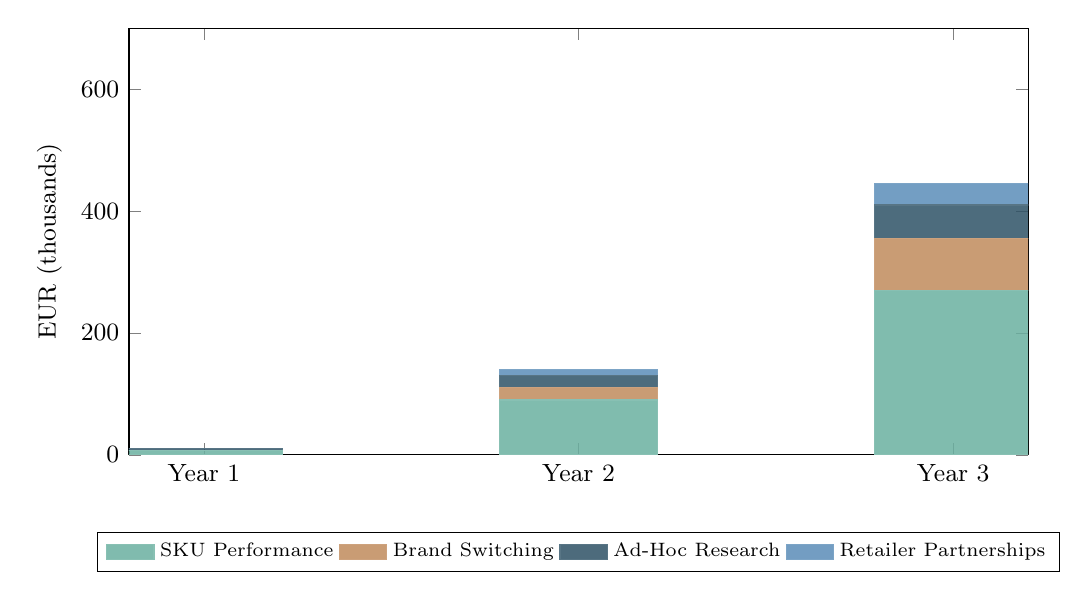
\begin{tikzpicture}
\begin{axis}[
  ybar stacked,
  width=13cm,
  height=7cm,
  bar width=2cm,
  ymin=0,
  ymax=700,
  ylabel={EUR (thousands)},
  ylabel style={font=\small},
  symbolic x coords={Year 1, Year 2, Year 3},
  xtick=data,
  tick label style={font=\small},
  legend style={at={(0.5,-0.18)}, anchor=north, legend columns=4, font=\scriptsize},
  area legend,
  every axis plot/.append style={fill opacity=0.85}
]
\addplot[fill=miloaccent, draw=miloaccent!80] coordinates {(Year 1, 7.5) (Year 2, 90) (Year 3, 270)};
\addplot[fill=milowarm, draw=milowarm!80] coordinates {(Year 1, 0) (Year 2, 20) (Year 3, 85)};
\addplot[fill=miloprimary, draw=miloprimary!80] coordinates {(Year 1, 3.5) (Year 2, 20) (Year 3, 55)};
\addplot[fill=miloblue, draw=miloblue!80] coordinates {(Year 1, 0) (Year 2, 10) (Year 3, 35)};
\legend{SKU Performance, Brand Switching, Ad-Hoc Research, Retailer Partnerships}
\end{axis}
\end{tikzpicture}
\end{center}

\subsection{Path to Profitability}

\begin{alertbox}
\textbf{Break-even point:} Late Year 2 to early Year 3 with 30+ paying B2B subscribers and growing retailer partnership revenue. By Year 3, the business approaches profitability with \texteuro{}260K--630K in B2B data revenue. The key lever is B2B client count: each additional client adds high-margin recurring revenue against a largely fixed panel cost base.
\end{alertbox}

\subsection{Unit Economics at Scale (Year 3)}

\begin{center}
\renewcommand{\arraystretch}{1.4}
\begin{tabularx}{\textwidth}{L{5.5cm} R{3cm} L{5cm}}
\toprule
\rowcolor{tabheader}
\textbf{\color{white}Metric} & \textbf{\color{white}Value} & \textbf{\color{white}Note} \\
\midrule
Avg.\ B2B contract value & \texteuro{}500/mo & Weighted across SMB to enterprise \\
\rowcolor{tabrow}
B2B revenue per panelist & \texteuro{}17--28/yr & Improves with scale \\
Effective reward cost per user & \texteuro{}7--10/yr\textsuperscript{*} & After redemption rates \\
\rowcolor{tabrow}
Revenue per user (blended) & \texteuro{}14--28/yr & B2B data revenue attributed per panelist \\
\rowcolor{tabrow}
\textbf{LTV:CAC ratio} & \textbf{3.5--6$\times$} & At 36-month retention \\
\bottomrule
\end{tabularx}
\end{center}

{\small\textsuperscript{*}Effective cost after accounting for coupon redemption rate ($\sim$50--60\%) and retailer partnership subsidies.}

\clearpage

% ============================================================================
% 13. FUNDING REQUEST
% ============================================================================
\section{Funding Request}

\subsection{The Ask: \texteuro{}150,000 -- \texteuro{}250,000 Seed Round}

\begin{center}
\renewcommand{\arraystretch}{1.5}
\begin{tabularx}{\textwidth}{L{4.5cm} R{3cm} L{6cm}}
\toprule
\rowcolor{tabheader}
\textbf{\color{white}Category} & \textbf{\color{white}Amount} & \textbf{\color{white}Details} \\
\midrule
User Acquisition (40\%) & \texteuro{}60K--100K & Paid social, influencer partnerships, referral program, App Store marketing \\
\rowcolor{tabrow}
Panel Rewards (25\%) & \texteuro{}37.5K--62.5K & Receipt rewards, spin wheel prizes, streak bonuses, coupon funding \\
Infrastructure (15\%) & \texteuro{}22.5K--37.5K & Gemini API, Railway hosting, Firebase, Android development \\
\rowcolor{tabrow}
B2B Go-to-Market (10\%) & \texteuro{}15K--25K & Sample reports, Datarade listing, industry events, B2B sales \\
Working Capital (10\%) & \texteuro{}15K--25K & Legal, accounting, contingency \\
\midrule
\textbf{Total} & \textbf{\texteuro{}150K--250K} & \\
\bottomrule
\end{tabularx}
\end{center}

\subsection{18-Month Milestones}

\begin{center}
\renewcommand{\arraystretch}{1.3}
\begin{tabularx}{\textwidth}{C{2.5cm} L{11cm}}
\toprule
\rowcolor{tabheader}
\textbf{\color{white}Milestone} & \textbf{\color{white}Target} \\
\midrule
Month 3 & 1,000 active panelists; iOS app live in App Store; first 500K receipt items in database \\
\rowcolor{tabrow}
Month 6 & 3,000 active panelists; first sample category reports; 10+ qualified B2B leads; gamification fully synced to backend \\
Month 9 & 5,000 active panelists; 8+ paying B2B subscribers; \texteuro{}3K--5K MRR; Android beta launch \\
\rowcolor{tabrow}
Month 12 & 8,000 active panelists; 15+ B2B clients; \texteuro{}8K--15K MRR; Netherlands expansion prep \\
Month 18 & 15,000+ panelists; 30+ B2B clients; Android live; retailer partnerships active; path to \texteuro{}200K+ ARR \\
\bottomrule
\end{tabularx}
\end{center}

\subsection{Alternative \& Complementary Funding}

\begin{itemize}[leftmargin=1.5em, itemsep=3pt]
  \item \textbf{Vlaio (Flanders):} \texteuro{}25K--50K non-dilutive grants for data/AI innovation projects\textsuperscript{[19]}
  \item \textbf{Innoviris (Brussels):} Up to \texteuro{}100K Proof of Business grants; up to \texteuro{}500K Innovative Starters Award\textsuperscript{[20]}
  \item \textbf{imec.istart:} \texteuro{}50K--200K pre-seed program (6\% equity)\textsuperscript{[21]}
  \item \textbf{BeAngels / BAN Vlaanderen:} \texteuro{}50K--100K angel investment
  \item \textbf{FMCG brand partnership:} A mid-size brand funds rewards in exchange for exclusive early data access
  \item \textbf{Pre-sales:} Letters of intent from 5--10 food producers to validate demand
\end{itemize}

\clearpage

% ============================================================================
% 14. RISK ANALYSIS
% ============================================================================
\section{Risk Analysis \& Mitigation}

\begin{center}
\renewcommand{\arraystretch}{1.4}
\begin{tabularx}{\textwidth}{L{3.5cm} C{1.5cm} C{1.5cm} L{6.5cm}}
\toprule
\rowcolor{tabheader}
\textbf{\color{white}Risk} & \textbf{\color{white}Severity} & \textbf{\color{white}Probability} & \textbf{\color{white}Mitigation} \\
\midrule
Insufficient user sign-ups & High & Medium & Multi-channel acquisition; generous rewards; referral program; app quality as differentiator \\
\rowcolor{tabrow}
User churn (stop submitting) & High & Medium & Five-layer gamification (wallet, streaks, tiers, badges, spins); app utility beyond receipt submission \\
Reward costs exceed revenue & Medium & Medium & Virtual wallet delays cash outflow; retailer partnerships subsidize coupons; adjustable reward rates \\
\rowcolor{tabrow}
Panel not representative & Medium & Medium & Demographic weighting; transparent methodology; Belgium-specific calibration \\
AI extraction quality issues & Medium & Medium & Monitor brand/category consistency; maintain alias tables; human QA sampling \\
\rowcolor{tabrow}
Slow B2B sales cycle & Medium & Medium & Free sample reports as lead gen; Datarade listing; industry events \\
App Store rejection & Low & Low & Full compliance with Apple/Google guidelines; no manipulative dark patterns \\
\rowcolor{tabrow}
YouGov drops their price & High & Very Low & Hasn't happened in 60+ years\textsuperscript{[22]}; Milo still 10--100$\times$ cheaper \\
GDPR compliance issues & High & Low & Aggregated data only; explicit consent; DPA alignment; regular audits \\
\rowcolor{tabrow}
Competing receipt app enters Belgium & Medium & Low & First-mover advantage; historical data compounds; deep Belgium-specific features \\
\bottomrule
\end{tabularx}
\end{center}

\clearpage

% ============================================================================
% 15. WHY NOW, WHY BELGIUM, WHY MILO
% ============================================================================
\section{Why Now, Why Belgium, Why Milo}

\subsection{Why Now}

\begin{itemize}[leftmargin=1.5em, itemsep=4pt]
  \item \textbf{AI-powered receipt extraction is now viable:} Google Gemini can extract structured data from receipts with high accuracy at minimal cost --- this was not possible even 2 years ago. Combined with Daltix product matching, extracted items resolve to real EAN codes with full product attributes.
  \item \textbf{Post-inflation budget awareness:} Belgian consumers experienced 12--15\% food inflation in 2022--2023.\textsuperscript{[4]} Demand for grocery budgeting tools has never been higher.
  \item \textbf{Privacy-first data economy:} With cookie deprecation and GDPR tightening, consumer-permissioned first-party data is the future. Milo is built for this world.
  \item \textbf{No European Byzzer:} NielsenIQ proved the SMB data market is massive, but their affordable product exists only in the US.\textsuperscript{[14]}
  \item \textbf{Mobile-first consumers:} Belgian smartphone penetration exceeds 90\%.\textsuperscript{[15]} The infrastructure for digital receipt adoption is universal.
  \item \textbf{Algori proves the European model works:} A Spanish receipt panel company raised \texteuro{}7.5M and signed 30+ FMCG brand clients.\textsuperscript{[23]} Belgium is next.
\end{itemize}

\subsection{Why Belgium}

\begin{itemize}[leftmargin=1.5em, itemsep=4pt]
  \item \textbf{Concentrated market:} 5 retailers control 85\%+ of grocery\textsuperscript{[5]} --- efficient to capture the entire market with a panel of 25K--50K households.
  \item \textbf{High PL share ($\sim$40\%):}\textsuperscript{[16]} Creates intense data demand from national brands defending share against private label encroachment.
  \item \textbf{Structural data gap:} Retailer data silos + expensive YouGov = a permanent, structurally defensible opportunity.
  \item \textbf{3,979 food companies:}\textsuperscript{[2]} Massive underserved TAM of SMB food producers with zero data access.
  \item \textbf{Trilingual launchpad:} Belgium's Dutch/French/English market provides a natural bridge to the Netherlands and France.
\end{itemize}

\subsection{Why Milo}

\begin{itemize}[leftmargin=1.5em, itemsep=4pt]
  \item \textbf{Free panelist model:} A genuinely useful consumer app funds itself through B2B data revenue --- no subscriptions, no paywalls, no friction.
  \item \textbf{Product-first approach:} Milo is designed to be a product users love, not a bare-bones data collection tool. This produces better data and higher retention.
  \item \textbf{Unique positioning:} The only affordable, cross-retailer, SKU-level consumer panel in Belgium with brand switching intelligence. No one else occupies this position.
  \item \textbf{Technology-first:} AI-powered extraction from day one. Native iOS with premium UX. Digital receipts only --- no camera scanning, no barcode scanning, no manual entry.
  \item \textbf{Capital-efficient:} \texteuro{}150K--250K seed round to reach self-sustaining dual revenue. No need for massive capital raises.
  \item \textbf{Compounding moat:} Every month of data increases the historical value of the dataset. By Month 12, Milo has the only longitudinal cross-retailer dataset in Belgium.
  \item \textbf{Solo founder, full-stack execution:} Product, iOS app, backend, AI pipeline, Daltix integration, data products, and business strategy built by one person. Capital goes to growth, not salaries.
\end{itemize}

\clearpage

% ============================================================================
% SOURCES
% ============================================================================
\section{Sources \& References}

{\small All market data and competitive claims in this document are substantiated by the following sources. Numbers marked with superscript references {\scriptsize [n]} throughout this document correspond to the entries below.}

\vspace{0.5em}

\begin{enumerate}[leftmargin=1.5em, itemsep=2pt, font=\small]
  \item[\textbf{[1]}] \textbf{Statbel} --- ``Structure of the Population,'' January 1, 2025. Belgium had 5,199,324 private households. \textit{statbel.fgov.be}
  \item[\textbf{[2]}] \textbf{BoldData} --- ``Top FMCG Companies Belgium,'' 2025. 3,979 food manufacturing companies in Belgium, 99\% SMEs. Corroborated by Fevia (Belgian Food Industry Federation). \textit{bolddata.nl}
  \item[\textbf{[3]}] \textbf{YouGov / GfK Consumer Panel Services} --- Enterprise contracts typically run \texteuro{}100,000+/year. GfK sold its European Consumer Panel business to YouGov in 2023 for \texteuro{}315M. Two-thirds of CPS revenues are recurring, with avg.\ contract length of 3 years. \textit{business.yougov.com}; Research Live, 2023.
  \item[\textbf{[4]}] \textbf{Trading Economics / Statbel CPI} --- Belgian food inflation peaked at 12--15\% in 2022, moderated to 8--10\% in 2023, and declined to 0.44\% by January 2026. \textit{tradingeconomics.com/belgium/food-inflation}; \textit{statbel.fgov.be}
  \item[\textbf{[5]}] \textbf{ESM Magazine / Statista} --- ``Top 10 Supermarket Chains in Belgium.'' Colruyt Group $\sim$25--26\%, Ahold Delhaize $\sim$21--23\%, Carrefour $\sim$18\%, Lidl $\sim$10\%, Aldi $\sim$9\%. Combined top-5 exceed 85\% market share. Market blindness percentages derived from these shares. \textit{esmmagazine.com}; \textit{statista.com}
  \item[\textbf{[6]}] \textbf{NielsenIQ Retail Spend Barometer Belgium} --- Belgian FMCG market \texteuro{}9.4B quarterly (Q3 2024), implying $\sim$\texteuro{}37--38B annual market. \textit{nielseniq.com}
  \item[\textbf{[7]}] \textbf{Colruyt Group Insights} --- $\sim$3 million households, $\sim$150 million transactions/year from Xtra loyalty card. Only covers Colruyt, OKay, and Spar stores. \textit{insights.colruytgroup.com}
  \item[\textbf{[8]}] \textbf{Media Marketing Delhaize (MMD) / Enlight+} --- 3M+ SuperPlus loyalty profiles. Transactional data limited to Delhaize stores. Part of Ahold Delhaize (\texteuro{}500M+ group ad/data revenue). \textit{mediamarketingdelhaize.be}
  \item[\textbf{[9]}] \textbf{Carrefour Links} --- 80M customers globally, 8B transactions. Built with Criteo, Google, LiveRamp. Belgium operations cover 2.4M loyalty card consumers. \textit{carrefour.com}; LiveRamp, 2023.
  \item[\textbf{[10]}] \textbf{Fetch Rewards} --- Valued at \$2.5B+ (PitchBook, 2024). 12.5M monthly active users, 11M receipts scanned per day, \$500M annual revenue run rate. \textit{PRNewswire}, ``Fetch Reports Strong Momentum for 2025,'' 2025.
  \item[\textbf{[11]}] \textbf{Ibotta Inc.} --- Q4/FY2024 Financial Results: \$367.3M revenue (+15\% YoY). IPO April 2024 (NYSE: IBTA). 50M+ app downloads. \textit{investors.ibotta.com}
  \item[\textbf{[12]}] \textbf{Foxintelligence / NielsenIQ} --- Acquired by NielsenIQ, now integrated as ``Digital Purchases by NIQ.'' Originally 600K-person e-receipt panel across Western Europe. Research Live, 2022. \textit{nielseniq.com}
  \item[\textbf{[13]}] \textbf{Shopmium} --- 10M+ downloads globally (mainly UK/France). Nielsen DaaS partnership for data activation. Data is biased toward promoted products only. \textit{shopmium.com}; CXNetwork; \textit{microsites.nielsen.com}
  \item[\textbf{[14]}] \textbf{NielsenIQ Byzzer} --- Self-service platform for small CPG brands, \$5K--10K/year. US-only; no equivalent exists in Belgium or Europe. Part of NielsenIQ (\$3.5B global revenue). \textit{nielseniq.com/global/en/products/byzzer}
  \item[\textbf{[15]}] \textbf{Statista / DataReportal} --- Belgian smartphone penetration: 92--97\% (2024--2025). \textit{statista.com}; DataReportal, ``Digital 2025: Belgium.''
  \item[\textbf{[16]}] \textbf{Statista / RetailDetail EU} --- Belgian private label food market share $\sim$40\%. Belgium has one of the highest PL shares in Europe. \textit{statista.com}; \textit{retaildetail.eu}
  \item[\textbf{[17]}] \textbf{IBISWorld / MarketLine} --- Belgian food \& grocery retail market $\sim$\texteuro{}47.9B (2025 estimate). \textit{ibisworld.com}; MarketLine Belgium Food \& Grocery report.
  \item[\textbf{[18]}] \textbf{Colruyt Group Annual Reports} --- FY 2024/25 revenue \texteuro{}10.96B (+1.1\% YoY). \textit{colruytgroup.com/investor-relations}
  \item[\textbf{[19]}] \textbf{VLAIO (Flanders Innovation \& Entrepreneurship)} --- Innovative Starters Support: \texteuro{}50K fixed grant. Development Projects: min.\ \texteuro{}25K, 25--50\% of approved costs. \textit{vlaio.be/en/subsidies}
  \item[\textbf{[20]}] \textbf{Innoviris (Brussels)} --- Proof of Business: up to \texteuro{}100K (50--70\% of expenses). Innovative Starters Award: up to \texteuro{}500K per project. Innovation Vouchers: up to \texteuro{}10K. \textit{innoviris.brussels}
  \item[\textbf{[21]}] \textbf{imec.istart} --- \texteuro{}50K cash + \texteuro{}50K convertible loan (up to \texteuro{}200K total) for 6\% equity. Ranked \#1 university-linked accelerator worldwide (UBI Global). \textit{imecistart.com}
  \item[\textbf{[22]}] \textbf{GfK / YouGov historical operations} --- GfK Consumer Panel Services has operated FMCG household panels across Europe since the 1960s (60+ years). No affordable self-service tier has ever been launched for small brands. Research Live, 2023.
  \item[\textbf{[23]}] \textbf{Algori.ai} --- ``Algori secures \texteuro{}3.6M to scale AI-driven shopper insights platform,'' December 2025. Panel statistics: 45,000 weekly active panelists, 25,000 daily baskets, 30+ FMCG brand clients, L'Or\'{e}al, Coca-Cola, Tetra Pak, Red Bull. \textit{algori.ai/news/algori-round-2025}
  \item[\textbf{[24]}] \textbf{Tech.eu} --- ``Algori raises \texteuro{}3.6M to scale its AI shopper insights platform globally,'' December 2025. Expansion plans (Poland, Germany, France), founder quotes, investor details. \textit{tech.eu/2025/12/09/algori-raises-eur36m-to-scale-its-ai-shopper-insights-platform-globally/}
  \item[\textbf{[25]}] \textbf{Startup Researcher} --- ``Algori Raises \texteuro{}3.6M for AI-Powered FMCG Data Platform,'' December 2025. Full funding history (\texteuro{}840K + \texteuro{}3.3M + \texteuro{}3.6M = \texteuro{}7.5M total), Jared Schrieber investor profile. \textit{startupresearcher.com/news/algori-raises-eur3-6-million-to-expand-ai-powered-fmcg-data-platform}
  \item[\textbf{[26]}] \textbf{Retail Tech Innovation Hub} --- ``Algori bags \texteuro{}3.6m to scale AI driven shopper insights platform,'' December 2025. Investor quotes from Pedro de Alava (Tech Transfer Agrifood) and Ricardo Jacinto (Shilling Capital). \textit{retailtechinnovationhub.com/home/2025/12/10/algori-bags-36m-to-scale-ai-driven-shopper-insights-platform-across-europe-and-latin-america}
  \item[\textbf{[27]}] \textbf{PROMOS App} --- Google Play Store listing (com.promos.app); firsthand testing March 2026. App mechanics: promo-gated model, camera-scan receipts, no base reward per receipt, rewards declining from \texteuro{}0.10 to \texteuro{}0.01. \textit{play.google.com/store/apps/details?id=com.promos.app}
  \item[\textbf{[28]}] \textbf{Trustpilot} --- PROMOS app reviews. Overall rating: 1.6/5. Complaints include reward rejections, opaque validation process, shrinking payouts, and misleading marketing claims. \textit{trustpilot.com}
  \item[\textbf{[29]}] \textbf{North Data} --- Promos Cupones Digitales S.L. trademark registration for ``ALGORI'' (word figurative mark), registered 21 April 2022. \textit{northdata.com}
\end{enumerate}

\clearpage

% ============================================================================
% CLOSING PAGE
% ============================================================================
\thispagestyle{empty}

\begin{tikzpicture}[remember picture, overlay]
  % Full page dark background
  \fill[milodark] (current page.south west) rectangle (current page.north east);

  % Subtle pattern
  \foreach \i in {1,...,10} {
    \draw[white, opacity=0.02, line width=0.3pt]
      ([xshift=\i*2.1cm]current page.south west) -- ([xshift=\i*2.1cm-4cm]current page.north west);
  }

  % Top accent line
  \fill[miloaccent] ([yshift=-0.6cm]current page.north west) rectangle ([yshift=-0.35cm]current page.north east);

  % Central message
  \node[anchor=center, text=white, font=\fontsize{20}{26}\selectfont\bfseries, text width=14cm, align=center] at ([yshift=3.5cm]current page.center) {Belgian consumers deserve better\\grocery insights.\\[6pt]Belgian brands deserve affordable\\market data.};

  \node[anchor=center, text=miloaccent, font=\fontsize{18}{24}\selectfont\bfseries] at ([yshift=1.2cm]current page.center) {Milo delivers both.};

  \node[anchor=center, text=white!60, font=\fontsize{10.5}{14}\selectfont, text width=12cm, align=center] at ([yshift=-0.3cm]current page.center) {One free app. One structurally defensible\\market position.};

  % Divider
  \draw[milowarm, line width=0.8pt] ([xshift=4cm, yshift=-1.4cm]current page.center) -- ([xshift=-4cm, yshift=-1.4cm]current page.center);

  % Logo
  \node[anchor=center] at ([yshift=-3.5cm]current page.center) {%
    
\includegraphics[width=3.5cm]{milo-logo.png}%
  };

  % Company name
  \node[anchor=center, text=white, font=\fontsize{32}{38}\selectfont\bfseries] at ([yshift=-6.3cm]current page.center) {MILO};

  % Tagline
  \node[anchor=center, text=miloaccent, font=\fontsize{11}{14}\selectfont] at ([yshift=-7.4cm]current page.center) {Consumer Panel \& Market Intelligence for Belgian FMCG};

  % Contact
  \node[anchor=center, text=white!80, font=\fontsize{10}{13}\selectfont\bfseries] at ([yshift=-8.6cm]current page.center) {Contact};
  \node[anchor=center, text=white!60, font=\fontsize{10}{13}\selectfont, align=center] at ([yshift=-9.6cm]current page.center) {Gilles Moenaert\\Founder\\Belgium};

  % Footer
  \node[anchor=center, text=white!40, font=\fontsize{8}{10}\selectfont] at ([yshift=1.5cm]current page.south) {This document is confidential and intended solely for the recipient. \copyright{} 2026 Milo. All rights reserved.};

  % Bottom accent line
  \fill[miloaccent] ([yshift=0.35cm]current page.south west) rectangle ([yshift=0.6cm]current page.south east);
\end{tikzpicture}

\end{document}
